\documentclass[aspectratio=169, 11pt]{beamer}

% Tema y colores
\usetheme{Madrid}
\usecolortheme{default}

% Paquetes esenciales para idioma y codificación
\usepackage[utf8]{inputenc}
\usepackage[spanish,es-tabla,es-noquoting]{babel}

% Matemáticas y gráficos
\usepackage{amsmath}
\usepackage{amsfonts}
\usepackage{amssymb}
\usepackage{graphicx}
\usepackage{tikz}
\usepackage{graphicx}      % Needed for \resizebox
\usepackage{circuitikz}    % Needed for the circuit environment
\usetikzlibrary{arrows.meta} % Needed for the Stealth arrows in your code
\usetikzlibrary{shapes,arrows,positioning,calc}
\usepackage{tikz-3dplot}
\usepackage{multirow}
\usepackage{booktabs}
\usepackage{colortbl}
% Hipervínculos
\usepackage{hyperref}
\setbeamertemplate{navigation symbols}{}
% Información del documento
\title{Análisis de la Red de Dependencias de Python}
\subtitle{Mundo interconectado. Una introducción práctica a la ciencia de las redes}
\author[B. Barañski \and J. Bengoa]{Bogurad Barañski Barañska \and Jorge Bengoa Pinedo}
\date{\today}

\begin{document}
	
	%---------------------------------------------------------
	\begin{frame}
		\titlepage
	\end{frame}
	
	%---------------------------------------------------------
	%\begin{frame}{Índice}
	%	\tableofcontents
	%\end{frame}
	
	%---------------------------------------------------------
	\section{Introducción}
	
%---------------------------------------------------------
	\begin{frame}{Construcción de la red}
		
		\begin{block}{Idea}
			Análisis del ecosistema de dependencias de Python. 
			\begin{itemize}
				\item \textbf{Nodos}: paquetes
				\item \textbf{Aristas}: dependencias
			\end{itemize}
		\end{block}
		
		\vspace*{-0.5cm}
		\begin{columns}[t]
			\begin{column}{0.48\textwidth}
				\begin{exampleblock}{Construcción de la Red}
					\begin{itemize}
						\item \textbf{Método}: \textit{web scraping} (API JSON de PyPI). 
						\item \textbf{Semillas}: 10 paquetes. 
						\item \textbf{Algoritmo}: búsqueda recursiva.
					\end{itemize}
				\end{exampleblock}
			\end{column}
			
			\begin{column}{0.48\textwidth}
				\begin{alertblock}{Entorno y Herramientas}
					\textbf{Hardware:} 
					\begin{itemize}
						\item i7-8750H | 16GB RAM | Win 11. 
					\end{itemize}
					\vspace{0.1cm}
					\textbf{Software Principal:} 
					\begin{itemize}
						\item \texttt{igraph} y \texttt{networkx}
						\item \texttt{vispy} y \texttt{matplotlib}
						\item \texttt{aiohttp} 
					\end{itemize}
				\end{alertblock}
			\end{column}
		\end{columns}
	\end{frame}
	
	%---------------------------------------------------------
	\begin{frame}{Objetivos del Estudio}
		\begin{enumerate}
			\item \textbf{Visión macroscópica} del ecosistema.
			\item Identificación de \textbf{hubs}.
			\item Segmentación de la red por \textbf{comunidades}.
			\item \textbf{Topología} de la red.
			\item \textbf{Visualización} mediante una herramienta interactiva propia.
		\end{enumerate}
	\end{frame}
		
	\begin{frame}{Descripción de la Red}
		\begin{block}{Grafo dirigido}
			\begin{itemize}
				\item $A \rightarrow B$: $A$ depende de $B$. 
				\item $A \to B \to C$: no hay arista $A \to C$.
			\end{itemize}
		\end{block}
		
		\begin{columns}[c]
			\begin{column}{0.4\textwidth}
				\begin{itemize}
					\item \textbf{Nodos}: 6765 
					\item \textbf{Aristas}: 36054 
					\item \textbf{Densidad}: 0,000788 (Muy baja) 
					\item \textbf{Clustering medio}: 0,3170 (Mundo pequeño perjudicado)
					\item \textbf{Clustering global}: 0,03584 (Grupos aislados)
				\end{itemize}
			\end{column}
			
			\begin{column}{0.5\textwidth}
				\begin{figure}
					\centering
					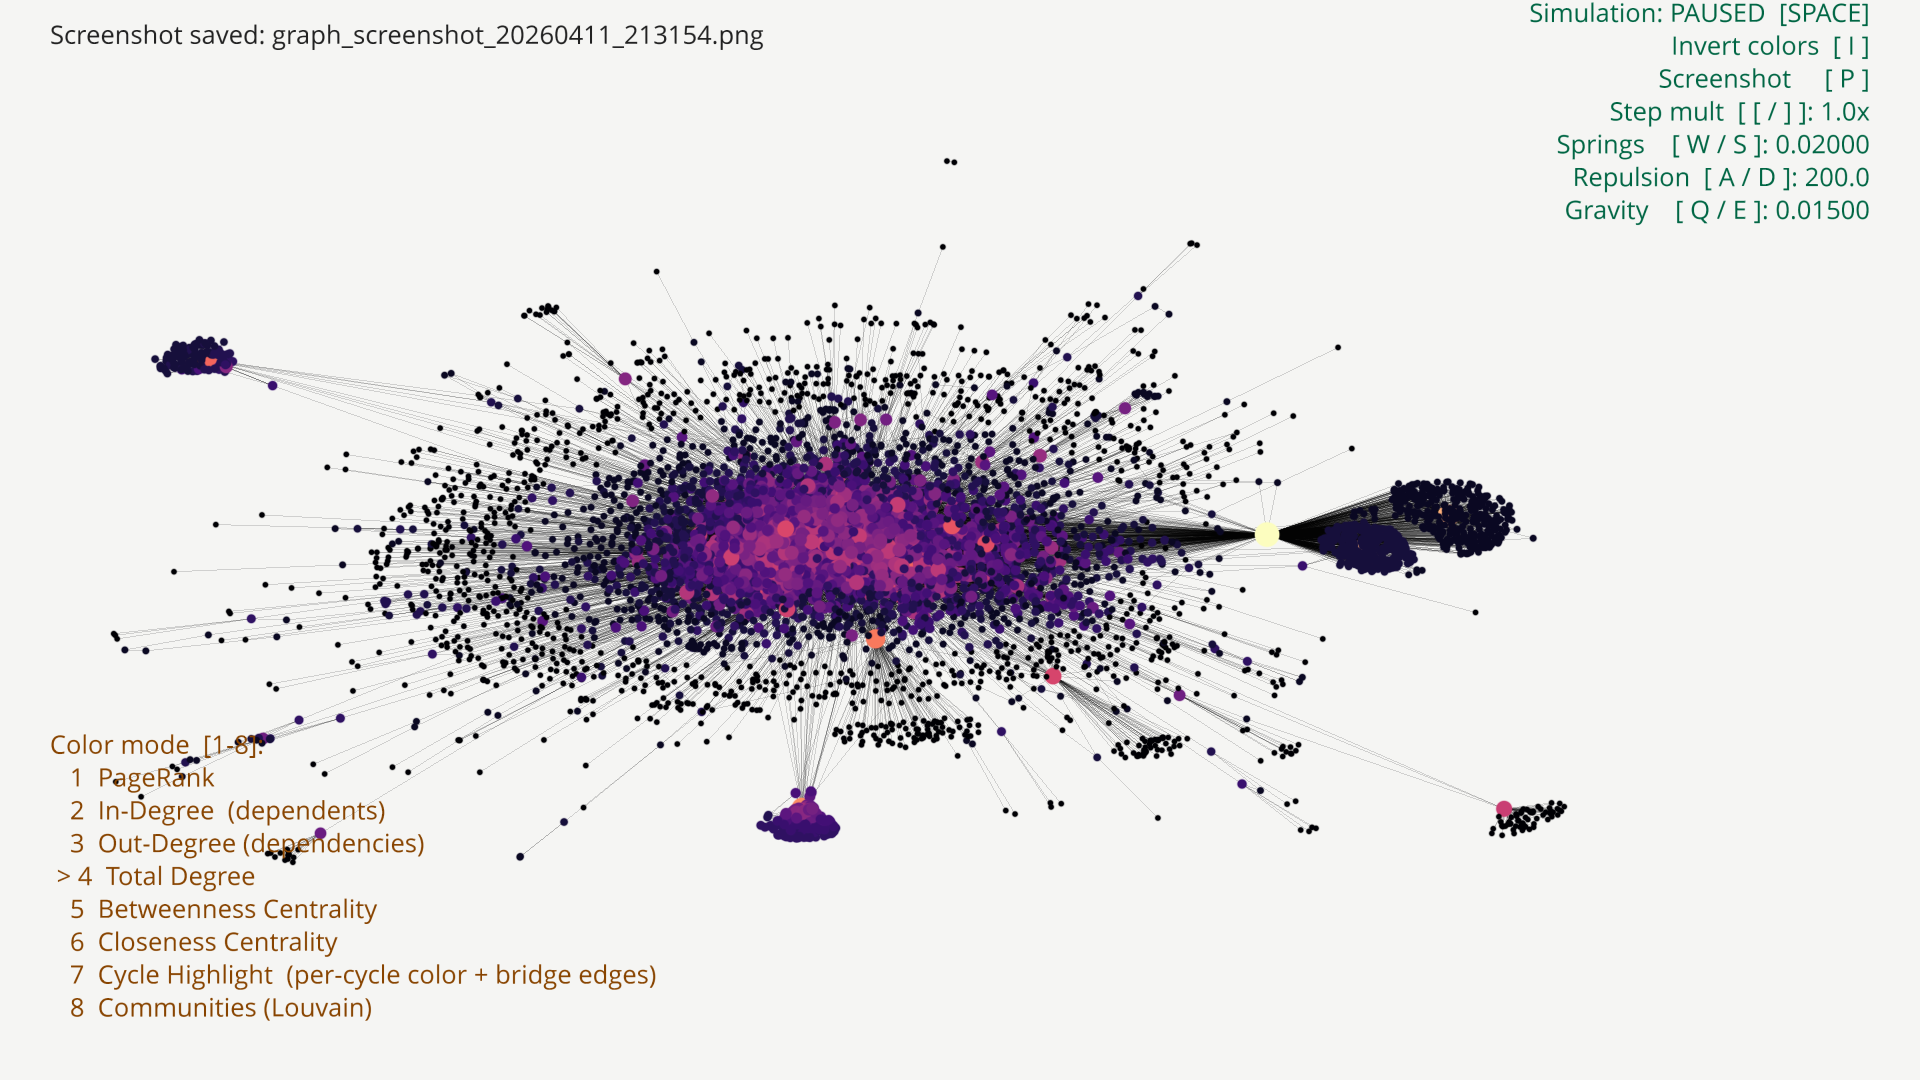
\includegraphics[width=1\linewidth]{Imagenes/TOTAL_ALL}
					\caption{Representación de la red a estudiar.}
				\end{figure}
			\end{column}
		\end{columns}
	\end{frame}
	
	\section*{Análisis de la red}
	\begin{frame}{Conectividad y Componente Gigante}
		\begin{columns}[c]		
			\begin{column}{0.45\textwidth}
				\begin{figure}
					\centering
					\includegraphics[width=1\linewidth]{Imagenes/ConectedComponent}
					\caption{Componente fuertemente conexa en rojo.}
				\end{figure}
			\end{column}
			
			\begin{column}{0.5\textwidth}
				\begin{block}{Tipos de conexión}
					\begin{itemize}
						\item \textbf{Débil}: ignora la dirección de aristas.
						\item \textbf{Fuerte}: ida y vuelta (ciclos).
					\end{itemize}
				\end{block}
				\begin{exampleblock}{Componente Gigante}
					\begin{itemize}
						\item \textbf{Tamaño}: 6763 nodos (99,97\%).
						\item \textbf{Nodos aislados}: \texttt{ansible} y \texttt{ansible-core}.
						\item \textbf{Motivo}: error del parser (regex)
					\end{itemize}
				\end{exampleblock}
			\end{column}
		\end{columns}
	\end{frame}
	
	\begin{frame}{Análisis de ciclos}
		\begin{columns}[c]
			\begin{column}{0.45\textwidth}
				\begin{itemize}
					\item \textbf{Componentes fuertemente conexas}: 3727.
					\item \textbf{Presencia de bucles}: instalaciones complejas y dependencias circulares.
					\item \textbf{Ciclo mayor}: 3038 paquetes.
					\item \textbf{Ciclo menor}: \texttt{ryd} $\leftrightarrow$ \texttt{ruamel.yaml}.
				\end{itemize}
			\end{column}
			
			\begin{column}{0.55\textwidth}
				\begin{figure}
					\centering
					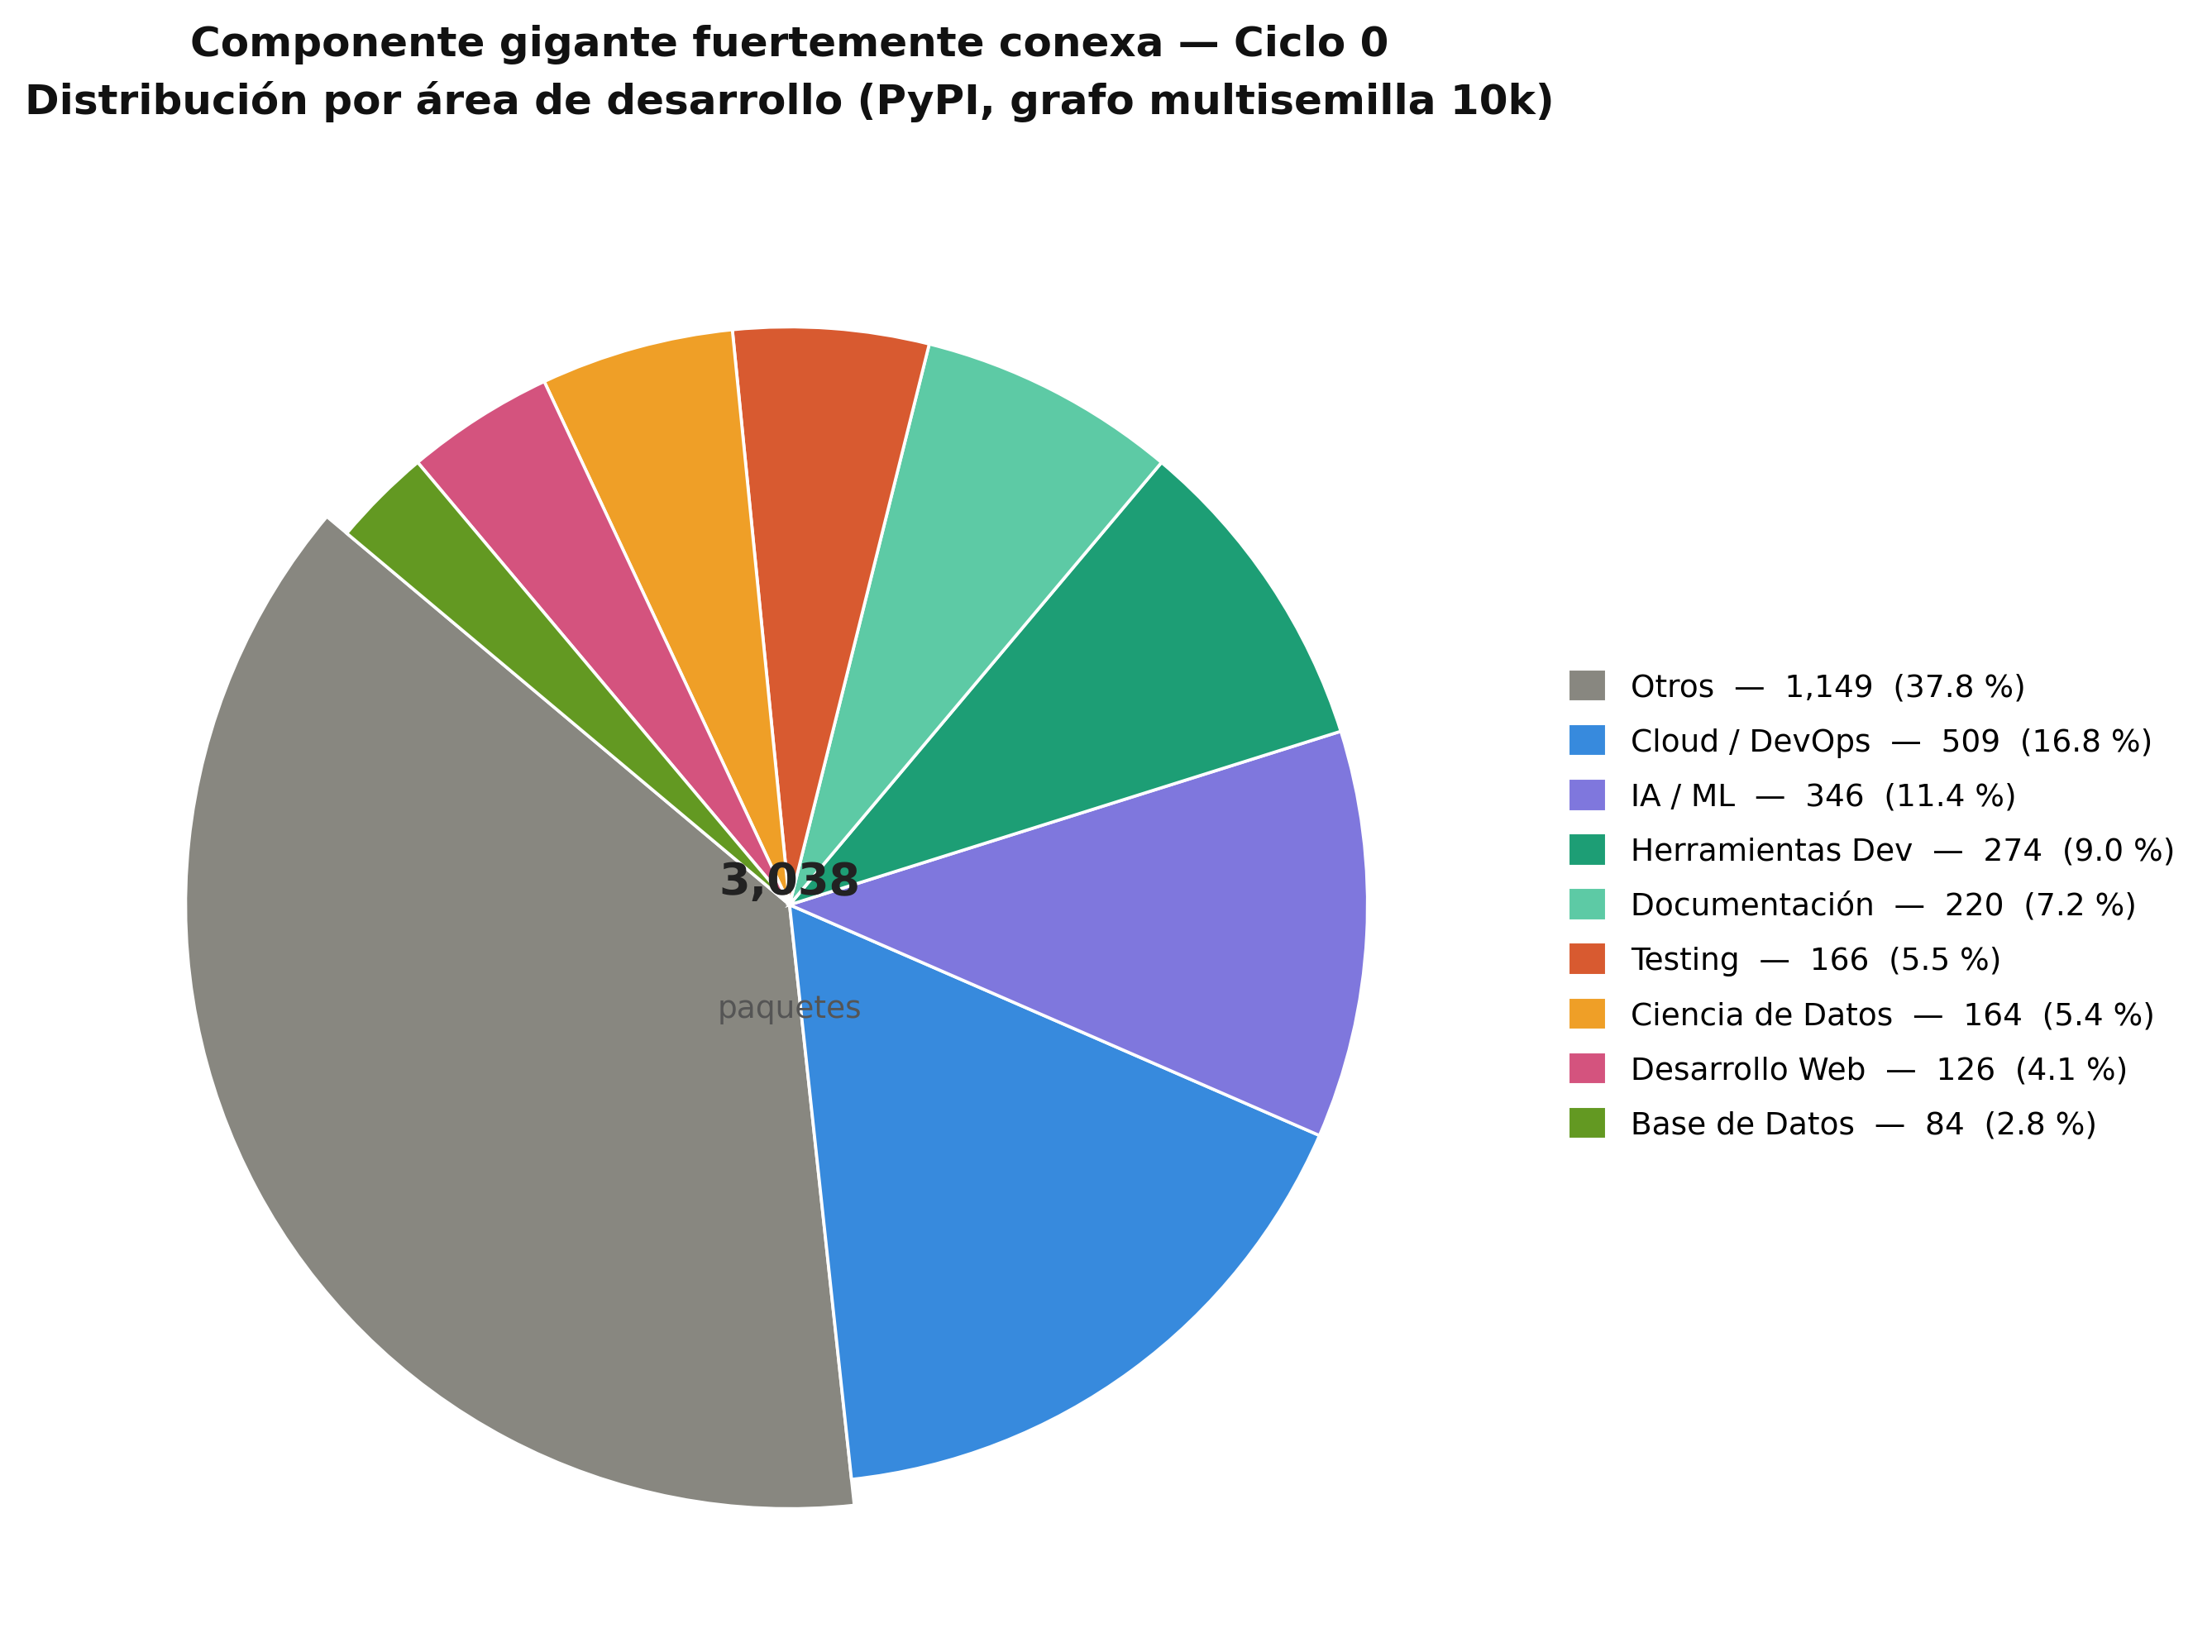
\includegraphics[width=0.9\linewidth]{Imagenes/pypi_ciclos_categorias.png}
					\caption{Distribución por áreas en el ciclo mayor.}
				\end{figure}
			\end{column}
		\end{columns}
	\end{frame}
	
	\begin{frame}{Distancias}
		\begin{block}{Profundidad de la red}
			\begin{description}
				\item[\textbf{Diámetro (25)}:] profundidad máxima de dependencias en el peor de los casos.
				\item[\textbf{Radio Entrada (6)}:] accesibilidad de los paquetes básicos (pasos para alcanzarlos).
				\item[\textbf{Radio Salida (13)}:] facilidad de instalación (profundidad mínima requerida).
			\end{description}
		\end{block}
		
		\begin{columns}
			\begin{column}{0.5\textwidth}
				\begin{figure}
					\centering
					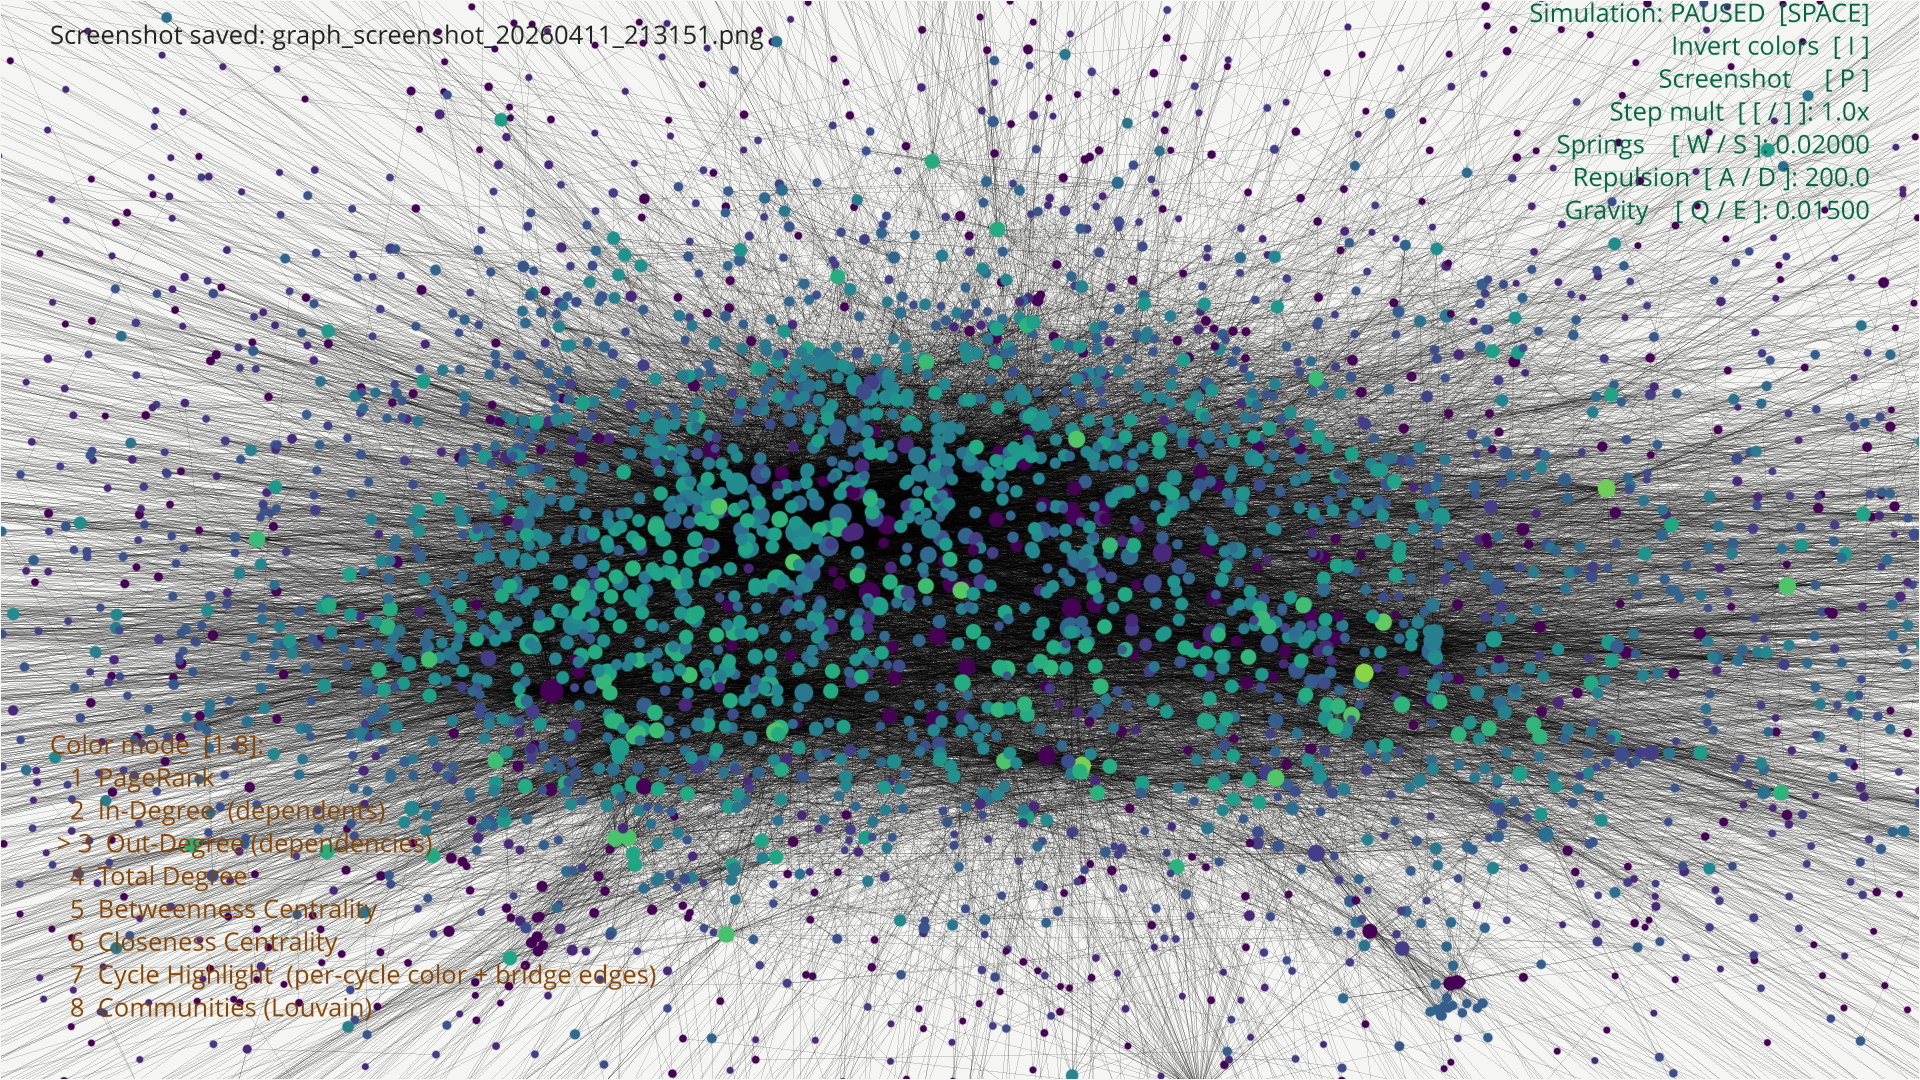
\includegraphics[width=0.8\linewidth]{Imagenes/OUT_center}
					\caption{Grado de salida.}
					\label{fig:outcenter}
				\end{figure}
			\end{column}
			\begin{column}{0.5\textwidth}
				\begin{figure}
					\centering
					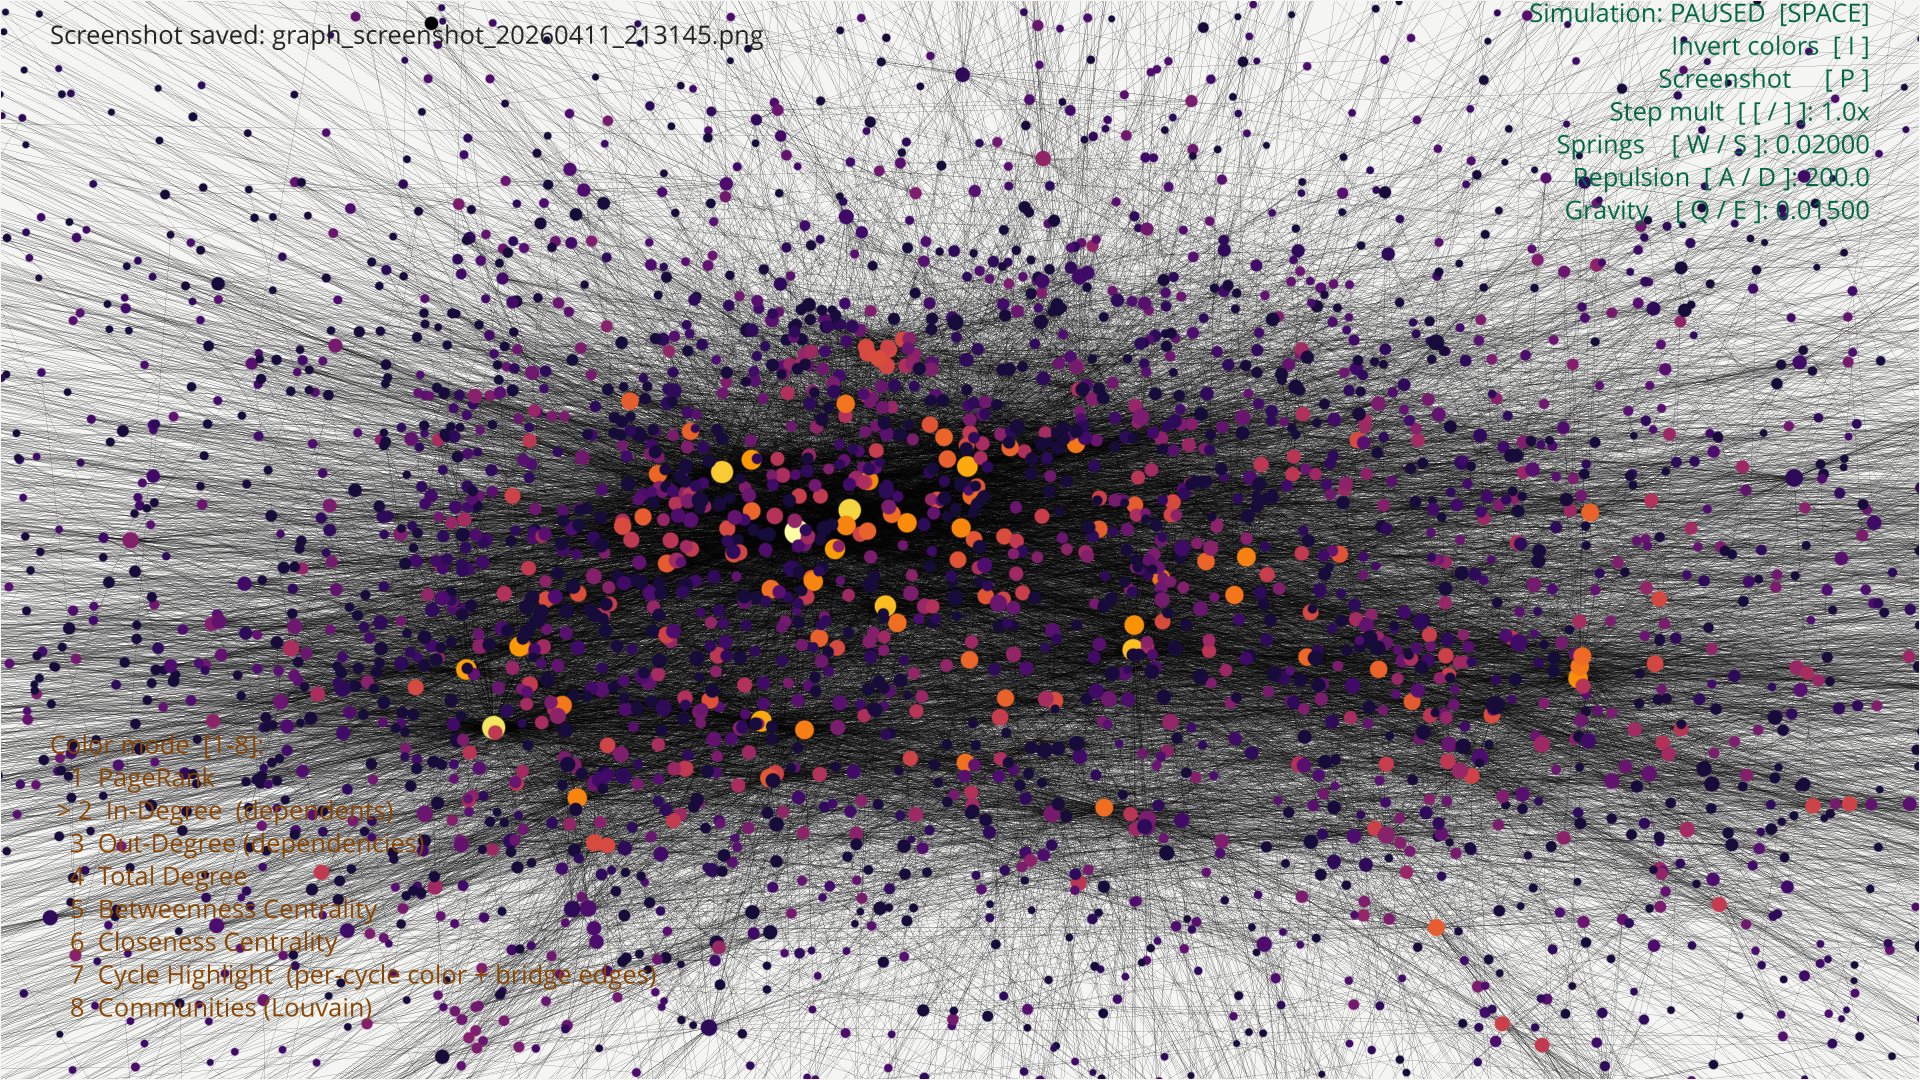
\includegraphics[width=0.8\linewidth]{Imagenes/IN_Center}
					\caption{Grado de entrada.}
					\label{fig:incenter}
				\end{figure}
			\end{column}
		\end{columns}
	\end{frame}
	
	%---------------------------------------------------------
	\begin{frame}{Distribución de grado y ley de potencias}
		\begin{columns}[T]
			
			% Columna Izquierda: Fórmulas MLE
			\begin{column}{0.5\textwidth}
				\begin{block}{Estimación de $\alpha$ (MLE)}
					Resolución de:
					\begin{equation*}
					\frac{\zeta'(\hat{\alpha}, x_{\min})}{\zeta(\hat{\alpha}, x_{\min})} = -\frac{1}{n} \sum_{i=1}^n \ln x_i
					\end{equation*}
					
					\vspace{0.2cm}
					
					Aproximación en tiempo discreto:
					\begin{equation*}
					\hat{\alpha} \approx 1 + n \left[ \sum_{i=1}^n \ln \frac{x_i}{x_{\min} - 0.5} \right]^{-1}
					\end{equation*}
				\end{block}
			\end{column}
			
			% Columna Derecha: KS y Bootstrapping
			\begin{column}{0.48\textwidth}
				\begin{exampleblock}{Estimación de $x_{\min}$}
					\textbf{1. Grid search:}
					\begin{itemize}
						\item Minimización de la distancia entre la distribución empírica $S(x)$ y la teórica $P(x)$:
					\end{itemize}
					\begin{equation*}
					KS = \max_{x \ge x_{\min}} |S(x) - P(x)|
					\end{equation*}
					
					\vspace{0.2cm}
					
					\textbf{2. Cálculo de Incertidumbre:}
					\begin{itemize}
						\item \textbf{Bootstrapping}.
						\item Conjuntos sintéticos para obtener la desviación típica de $\hat{x}_{\min}$.
					\end{itemize}
				\end{exampleblock}
			\end{column}
			
		\end{columns}
	\end{frame}
	
	%---------------------------------------------------------
	\begin{frame}{Test de bondad de ajuste}
		\begin{block}{¿Por qué?}
			\begin{itemize}
				\item Una realización aleatoria de una ley de potencias puede no parecerlo por el ruido.
				\item ¿Desviaciones por muestreo o porque los datos provienen de otra distribución?
			\end{itemize}
		\end{block}
		
		\vspace{-0.2cm}
		
		\begin{columns}[T]
			\begin{column}{0.48\textwidth}
				\begin{exampleblock}{Método semiparamétrico}
					\begin{itemize}
						\item Generación de datos sintéticos.
						\item Reajuste de $\hat{x}_{\min}$ y $\hat{\alpha}$.
						\item \textbf{p-valor:} proporción que el $KS$ de los datos sintéticos supera al empírico.
					\end{itemize}
				\end{exampleblock}
			\end{column}
			
			\begin{column}{0.48\textwidth}
				\begin{alertblock}{Muestreo (Cola)}
					Generación de la cola:
					\begin{equation*}
					P(x) = \sum_{x'=x}^{\infty} p(x') = 1 - r
					\end{equation*}
					Aproximación:
					\begin{equation*}
					x = \left\lfloor \left(x_{\min} - \frac{1}{2}\right) (1 - r)^{-\frac{1}{\alpha-1}} + \frac{1}{2} \right\rfloor
					\end{equation*}
				\end{alertblock}
			\end{column}
		\end{columns}
	\end{frame}
	
	%---------------------------------------------------------
	\begin{frame}{Comparación con hipótesis alternativas (Test de Vuong)}
		\begin{block}{Razón de log-verosimilitudes ($\mathcal{R}$)}
			¿Alguna distribución alternativa se ajusta mejor que la ley de potencias?
			\begin{equation*}
			\mathcal{R} = \sum_{i=1}^{n} [\ln p_1(x_i) - \ln p_2(x_i)] = \sum_{i=1}^{n} [\ell_i^{(1)} - \ell_i^{(2)}]
			\end{equation*}
		\end{block}
		
		\begin{columns}[t]
			\begin{column}{0.5\textwidth}
				\textbf{Interpretación:}
				\begin{itemize}
					\item $\mathcal{R} > 0$: ley de potencias favorable.
					\item $\mathcal{R} < 0$: alternativa favorable.
					\item $\mathcal{R} \approx 0$: no distinguibles.
				\end{itemize}
			\end{column}
			
			\begin{column}{0.5\textwidth}
				\textbf{Significancia estadística:}
				\footnotesize
				\begin{itemize}
					\item TCL: $\mathcal{R} \sim \mathcal{N}(\mu, \sigma^2)$, con $\sigma^2 \approx \hat{\sigma}^2$
					\item $H_0$: $\mathcal{R} \sim \mathcal{N}(0, \sigma^2)$
				\end{itemize}
				\begin{equation*}
				p = \frac{1}{\sqrt{2\pi n\sigma^2}} \left[ \int_{-\infty}^{-|\mathcal{R}|} e^{-\frac{t^2}{2n\sigma^2}} dt + \int_{|\mathcal{R}|}^{\infty} e^{-\frac{t^2}{2n\sigma^2}} dt \right]
				\end{equation*}
			\end{column}
		\end{columns}
	\end{frame}
	
	%---------------------------------------------------------
	\begin{frame}{Ajuste de ley de potencias}
		\begin{table}
			\centering
			\resizebox{0.9\linewidth}{!}{
				\begin{tabular}{lcc}
					\hline
					\textbf{Métrica} & \textbf{Grado de Entrada} & \textbf{Grado de Salida} \\
					\hline
					$x_{\min}$ óptimo & 3.0 & 11.0 \\
					$x_{\min}$ bootstrap & $3.6 \pm 1.4$ & $21.4 \pm 8.9$ \\
					$\alpha$ óptimo & $1.8999 \pm 0.0222$ & $2.5158 \pm 0.0479$ \\
					KS óptima & 0.0139 & 0.0608 \\
					$n_{\text{cola}}$ & 1646 (24.3\%) & 1001 (22.0\%) \\
					p-valor (Test KS) & \textbf{0.532} & \textbf{0.000} \\
					\hline
					Test de Vuong & No rechazada ($p > 0.1$) & Rechazada ($p \le 0.1$) \\
					\hline
				\end{tabular}
			}
			\caption{Resumen del ajuste para los grados de entrada y salida.}
		\end{table}
	\end{frame}
	
	%---------------------------------------------------------
	\begin{frame}{Distribuciones log-log y búsqueda de $x_{\min}$}
		\begin{figure}
			\centering
			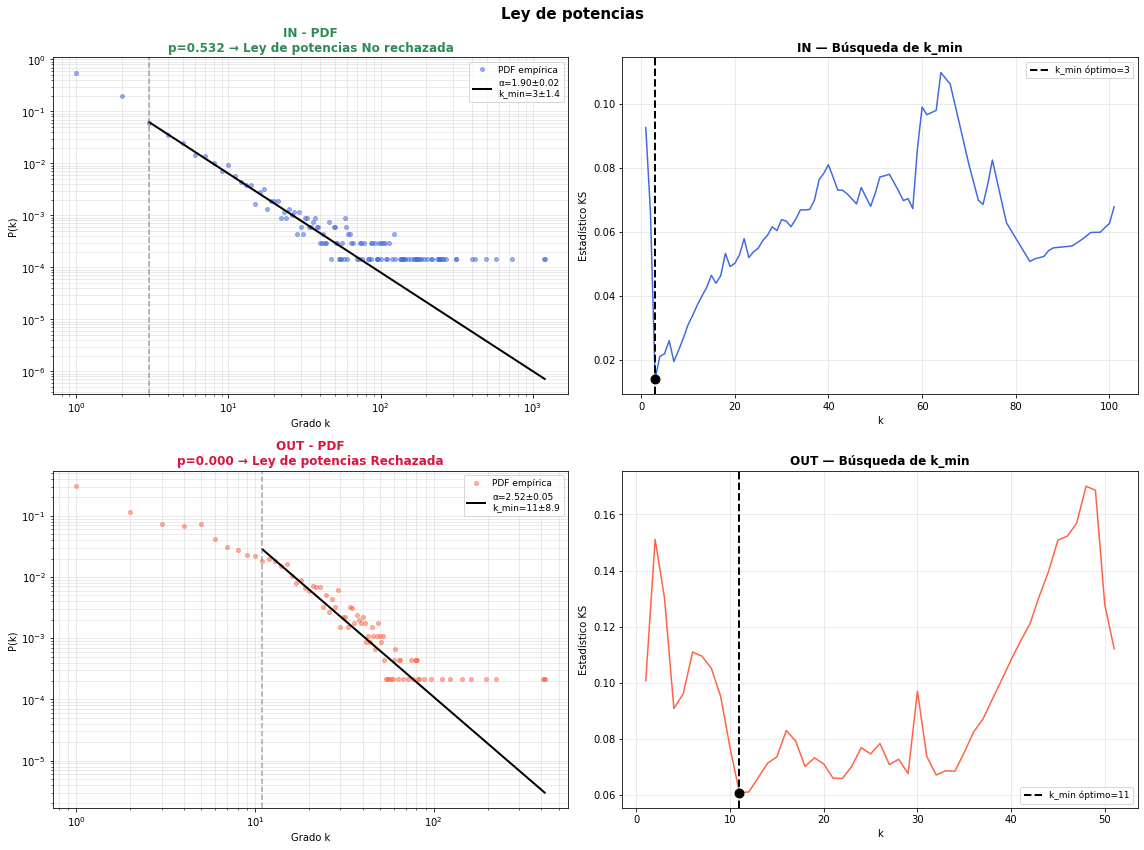
\includegraphics[width=\linewidth, height=0.65\textheight, keepaspectratio]{Imagenes/ley_potencias_kmin}
			\caption{Distribuciones de masa empíricas vs. teóricas y búsqueda de $x_{\min}$.}
		\end{figure}
	\end{frame}
	
	%---------------------------------------------------------
	\begin{frame}{Comparación con alternativas}
		\begin{table}
			\centering
			\resizebox{\linewidth}{!}{
				\begin{tabular}{lrcl}
					\hline
					\textbf{Distribución Alternativa} & \textbf{LR ($\mathcal{R}$)} & \textbf{p-valor} & \textbf{Interpretación} \\
					\hline
					\multicolumn{4}{c}{\textbf{Grado de Entrada} \quad ($k_{\min}=3, \alpha=1.900, p_{\text{KS}}=0.532$)} \\
					\hline
					Exponencial & $8.432$ & $<0.001$ & Ley de potencias favorable \\
					Poisson     & $5.401$ & $<0.001$ & Ley de potencias favorable \\
					Yule        & $-1.598$ & $0.110$ & No distinguibles \\
					\hline
					\multicolumn{4}{c}{\textbf{Grado de Salida} \quad ($k_{\min}=11, \alpha=2.516, p_{\text{KS}}<0.001$)} \\
					\hline
					Exponencial & $1.307$ & $0.191$ & No distinguibles \\
					Poisson     & $3.824$ & $<0.001$ & Ley de potencias favorable \\
					Yule        & $-8.943$ & $<0.001$ & Alternativa favorable \\
					\hline
				\end{tabular}
			}
			\caption{Tests de razón de verosimilitud frente a distribuciones alternativas.}
		\end{table}
	\end{frame}
	
\begin{frame}{Distribuciones de Centralidad}
	
	% Imagen en la parte superior, más grande
	\begin{figure}
		\centering
		% Ajusta el width o el height según lo necesites, keepaspectratio evita que se deforme
		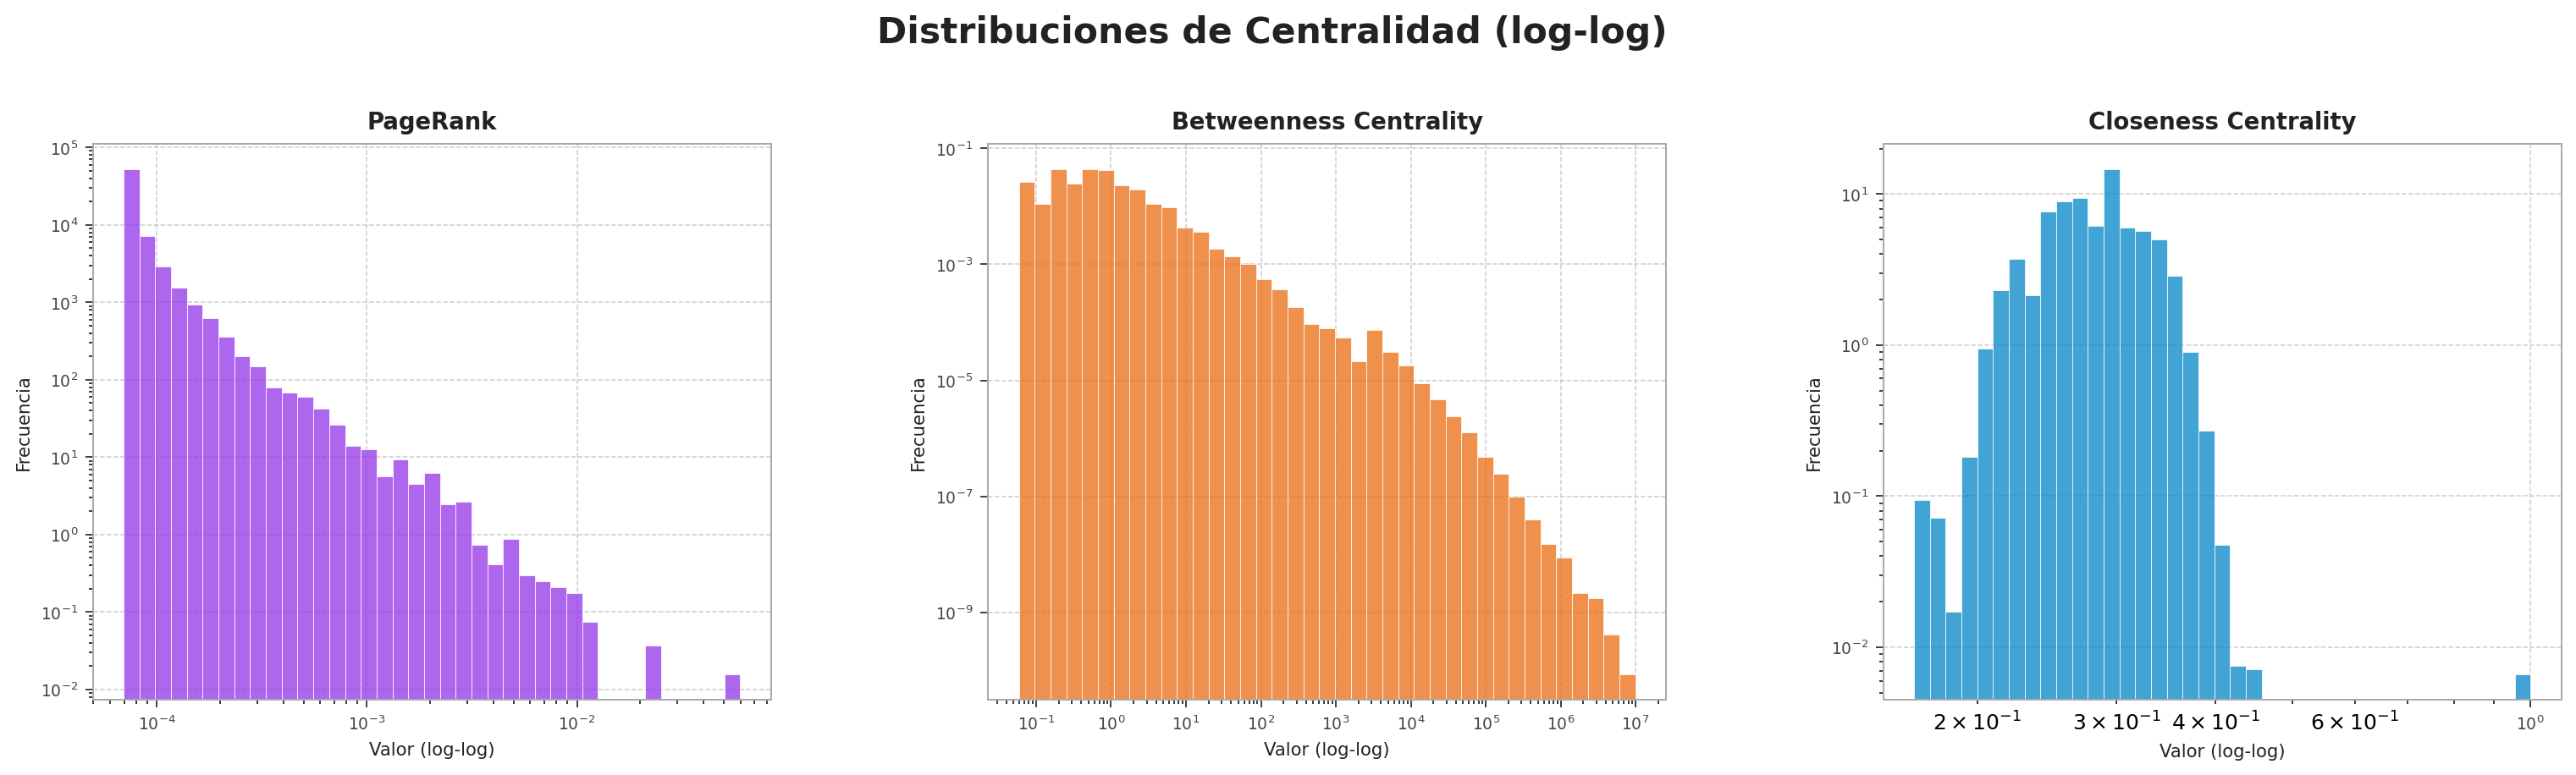
\includegraphics[width=0.9\textwidth, height=0.45\textheight, keepaspectratio]{Imagenes/centrality_distributions_loglog}
	\end{figure}
	
	\vspace{-0.2cm} % Reduce el espacio entre la imagen y las ecuaciones
	
	% Ecuaciones en la parte inferior, distribuidas en 3 columnas
	\begin{columns}[T]
		
		\begin{column}{0.33\textwidth}
			\centering
			\textcolor{structure}{\textbf{PageRank}}
			{\footnotesize
				\begin{equation*}
					\log(P(PR)) = -\gamma \log(PR) + C
				\end{equation*}
			}
			\vspace{-0.4cm}
			{\scriptsize \textit{Escenario rich get richer.}\par}
		\end{column}
		
		\begin{column}{0.33\textwidth}
			\centering
			\textcolor{structure}{\textbf{Intermediación}}
			{\footnotesize
				\begin{equation*}
					\log(P(CI)) \approx -K (\log CI)^2 + C
				\end{equation*}
			}
			\vspace{-0.4cm}
			{\scriptsize \textit{Exclusividad de los puentes.}\par}
		\end{column}
		
		\begin{column}{0.33\textwidth}
			\centering
			\textcolor{structure}{\textbf{Cercanía}}
			{\footnotesize
				\begin{equation*}
					P(CC) = \frac{1}{\sigma\sqrt{2\pi}} e^{-\frac{1}{2}\left(\frac{CC-\mu}{\sigma}\right)^2}
				\end{equation*}
			}
			\vspace{-0.4cm}
			{\scriptsize \textit{Fenómeno de Pequeño Mundo.}\par}
		\end{column}
		
	\end{columns}
	
\end{frame}
	\begin{frame}
		\centering
		\Huge \textbf{¡Muchas gracias por su atención!} \\
		\vspace{1cm}
		\Large ¿Preguntas?
	\end{frame}
	
	%---------------------------------------------------------
	% DIAPOSITIVA 1: Metodología y Hardware
	%---------------------------------------------------------
	%---------------------------------------------------------
	% DIAPOSITIVA 1: Metodología y Definición de Magnitudes
	%---------------------------------------------------------
	%---------------------------------------------------------
	% DIAPOSITIVA 1: Metodología y Definición de Magnitudes
	%---------------------------------------------------------
	%---------------------------------------------------------
	% DIAPOSITIVA 1: Fundamentos Matemáticos y Metodología
	%---------------------------------------------------------
	%---------------------------------------------------------
	% DIAPOSITIVA 1: Fundamentos Matemáticos y Metodología
	%---------------------------------------------------------
	%---------------------------------------------------------
	% DIAPOSITIVA 1: Metodología y Optimización (Corregida)
	%---------------------------------------------------------
	\begin{frame}{Metodología: Función de Coste y Optimización}
		
		\begin{block}{1. Función de Objetivo $\mathcal{L}(\theta)$}
			\[ \mathcal{L}(\theta) = \sum_{i \in \{in, out\}} W_1(P_i, \hat{P}_i) + 10 \cdot |\Delta C| + 10 \cdot |\Delta r| \]
			\vspace{-2mm}
			\begin{itemize}
				\item \textbf{Distancia $W_1$:} $\int |F_P(x) - F_{\hat{P}}(x)| \, dx$ \quad (Ajuste de distribución de grados)
				\item \textbf{Transitividad ($C$):} $C = \frac{3 \times \text{Tr}(A^3)}{\sum_{i,j} (A^2)_{ij}}$ \quad (Ajuste macro-estructural)
				\item \textbf{Reciprocidad ($r$):} $r = \frac{\text{Tr}(A^2)}{\sum_{i,j} A_{ij}}$ \quad (Ajuste de enlaces bidireccionales)
			\end{itemize}
		\end{block}
		
		\begin{block}{2. Estrategia de Búsqueda}
			Minimización del funcional $\mathcal{L}(\theta)$ mediante \textbf{Optimización Bayesiana} utilizando \textbf{Optuna}. Este estimador bayesiano infiere probabilísticamente las regiones óptimas del espacio de parámetros en lugar de realizar búsquedas aleatorias o en cuadrícula.
		\end{block}
		
	\end{frame}
	%---------------------------------------------------------
	% DIAPOSITIVA 2: Resultados del Entrenamiento (Ranking)
	%---------------------------------------------------------
	\begin{frame}{Resultados del Entrenamiento: Ranking de Modelos}
		\textbf{Hardware de Ejecución:}
		\begin{itemize}
			\item \textbf{CPU:} AMD Ryzen (Arquitectura Zen 3) @ 3.8 GHz
			\item \textbf{RAM:} 32 GB
		\end{itemize}
		\begin{table}
			\centering
			\resizebox{0.9\linewidth}{!}{
				\begin{tabular}{llcl}
					\toprule
					\textbf{Pos.} & \textbf{Modelo} & \textbf{Loss Final} & \textbf{Fortaleza Principal} \\
					\midrule
					\rowcolor{green!10} 1 & \textbf{BTER} & 4.902 & Excelente ajuste de grados y clustering. \\
					2 & \textbf{Copying} & 7.698 & El mejor replicando la forma de los hubs ($W_1$ in). \\
					3 & \textbf{Barabási-Albert} & 7.911 & Referencia sólida para crecimiento orgánico. \\
					4 & \textbf{Bianconi-BB} & 8.765 & Incorpora aptitud, pero inferior a la copia pura. \\
					5 & \textbf{ERGM} & 10.853 & Control total sobre reciprocidad y densidad. \\
					6 & \textbf{Kronecker} & 11.206 & Estructura fractal, pero demasiado rígida. \\
					7 & \textbf{SBM\_PA} & 11.631 & Falla al equilibrar comunidades y grados. \\
					\bottomrule
				\end{tabular}
			}
			\caption{Resultados tras 300 trials por modelo (Tiempo total: 01:15:17).}
		\end{table}
	\end{frame}
	
	%---------------------------------------------------------
	% DIAPOSITIVA 3: Validación Estadística (P-Values)
	%---------------------------------------------------------
	\begin{frame}{Validación Estadística: ¿Qué miden los P-valores?}
			\begin{itemize}
				\item \textbf{Max Hub:} Mide si el modelo genera paquetes tan populares como los reales (ej. \textit{numpy}).
				\item \textbf{Assortativity:} Mide si los paquetes populares dependen de otros populares (Lógica de ingeniería).
				\item \textbf{Significancia:} Un $p < 0.05$ (*) indica que el modelo es \textbf{estadísticamente diferente} a la realidad.
			\end{itemize}
		\begin{center}
			\footnotesize
			\begin{tabular}{lcccc}
				\hline
				\textbf{Modelo} & \textbf{Clust} & \textbf{Max Hub} & \textbf{Assort} & \textbf{Recip} \\
				\hline
				Copying & 0.013* & \textbf{0.252} & 0.007* & 0.013* \\
				BTER & 0.007* & 0.013* & 0.007* & 0.007* \\
				\hline
			\end{tabular}
		\end{center}
	\end{frame}
	
	%---------------------------------------------------------
	% DIAPOSITIVA 4: Análisis de Errores y Trade-offs
	%---------------------------------------------------------
	\begin{frame}{El Conflicto entre Micro y Macro Estructura}
		\begin{columns}
			\begin{column}{0.5\textwidth}
				\centering
				\textbf{Éxito en Micro-Escala} \\
				\vspace{2mm}
				\textit{Modelo Copying} \\
				Recluta nodos mediante imitación. \\
				\textbf{Resultado:} Capta perfectamente la distribución de grados de entrada ($p=0.252$).
			\end{column}
			\begin{column}{0.5\textwidth}
				\centering
				\textbf{Éxito en Macro-Escala} \\
				\vspace{2mm}
				\textit{Modelo BTER} \\
				Organiza nodos en bloques densos. \\
				\textbf{Resultado:} Es el único que se acerca al clustering real, aunque a costa de la forma de los hubs.
			\end{column}
		\end{columns}
		\vspace{4mm}
		\begin{alertblock}{Conclusión Técnica}
			Existe un \textbf{trade-off estructural}: Los modelos que mejor replican los hubs (Copying/BA) ignoran las comunidades, mientras que los que modelan comunidades (BTER/SBM) suelen distorsionar las colas de la distribución de grados.
		\end{alertblock}
	\end{frame}
	
	%---------------------------------------------------------
	% DIAPOSITIVA 5: Veredicto Final
	%---------------------------------------------------------
	\begin{frame}{Veredicto: La Naturaleza de PyPI}
		\begin{enumerate}
			\setlength\itemsep{1em}
			\item \textbf{Crecimiento por Imitación:} La red no es aleatoria. El alto desempeño del modelo \textit{Copying} sugiere que los desarrolladores eligen dependencias imitando a los paquetes exitosos.
			\item \textbf{Estructura Disasortativa:} Ningún modelo replicó la asortatividad. PyPI es disasortativo por diseño humano: grandes frameworks dependen de librerías pequeñas y utilitarias. Los algoritmos no entienden esta "lógica de software".
			\item \textbf{Hacia un Modelo Híbrido:} Para una réplica perfecta, se requeriría un modelo que combine el \textit{copying} para el crecimiento y una estructura de bloques (BTER) para las áreas temáticas de la librería.
		\end{enumerate}
	\end{frame}
	
	
	%---------------------------------------------------------
	% DIAPOSITIVA 1: Copying vs BA
	%---------------------------------------------------------
	\begin{frame}{Micro-Dinámicas: El Triunfo de la Copia}
		\begin{columns}
			\begin{column}{0.48\textwidth}
				\centering
				\textbf{Modelo Copying} \\
				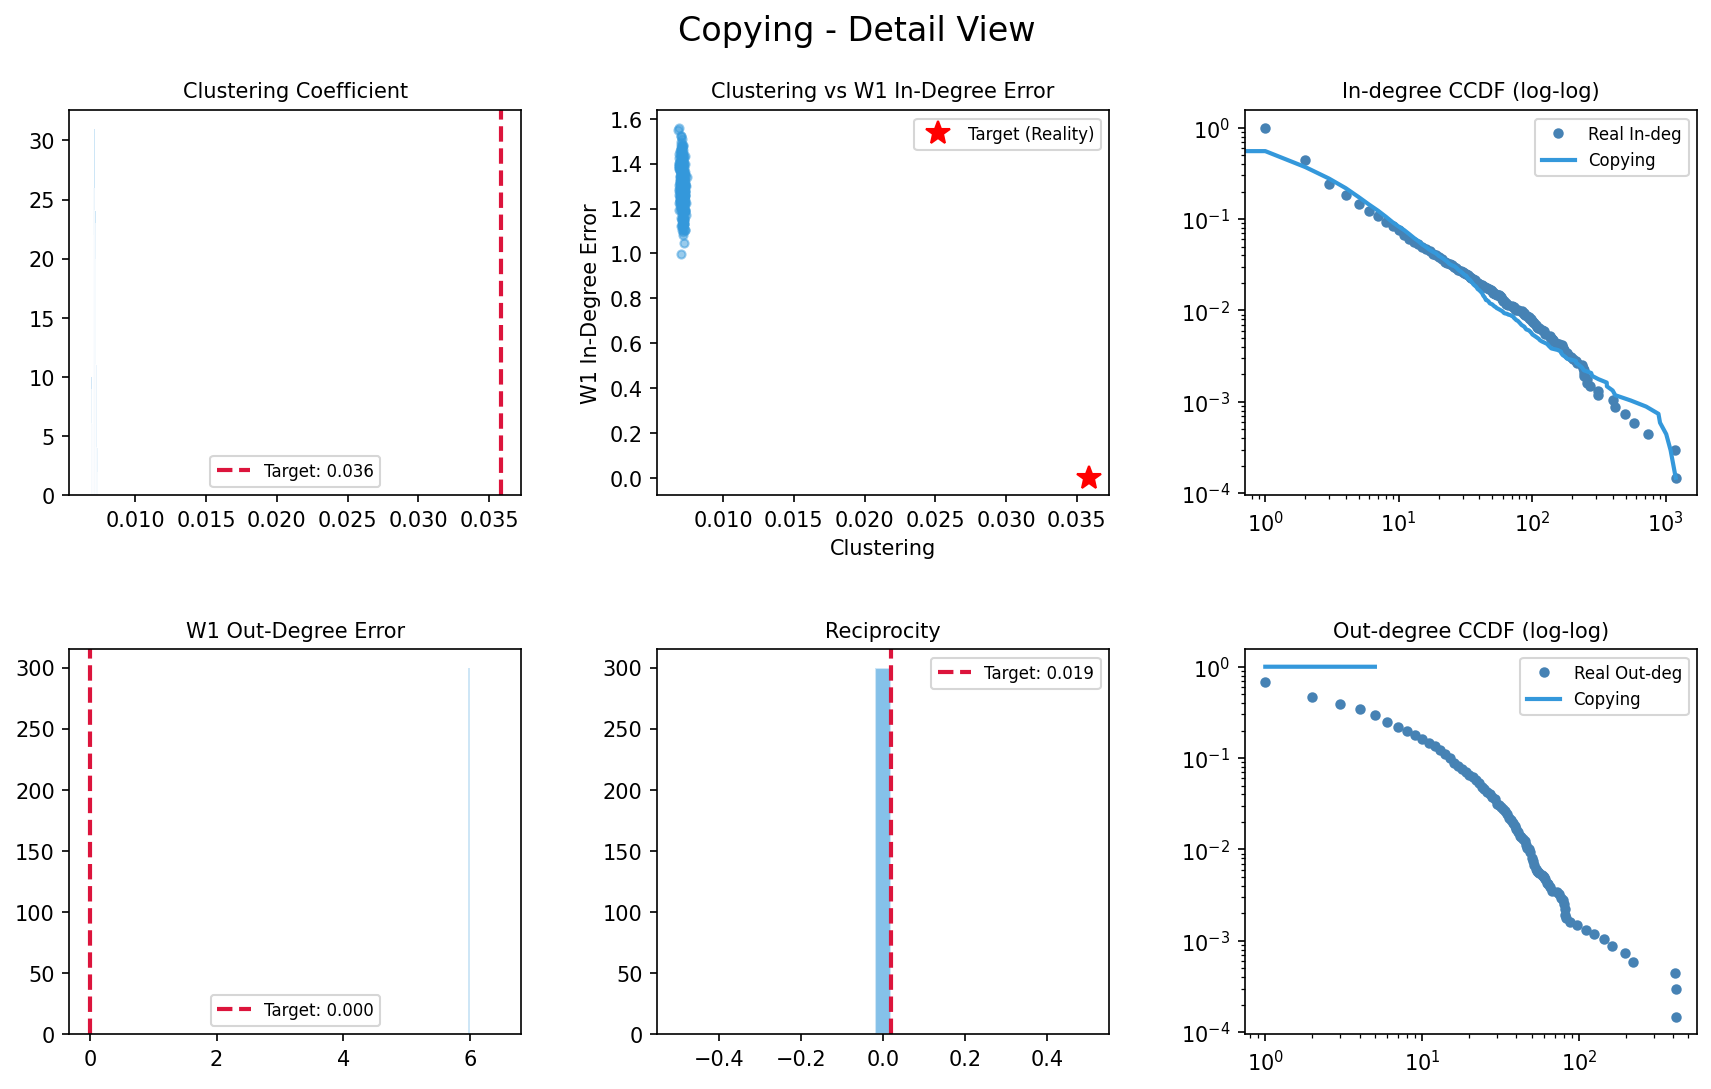
\includegraphics[width=\linewidth]{Imagenes/summary_Copying.png}
			\end{column}
			\begin{column}{0.48\textwidth}
				\centering
				\textbf{Modelo Barabási-Albert (Nulo)} \\
				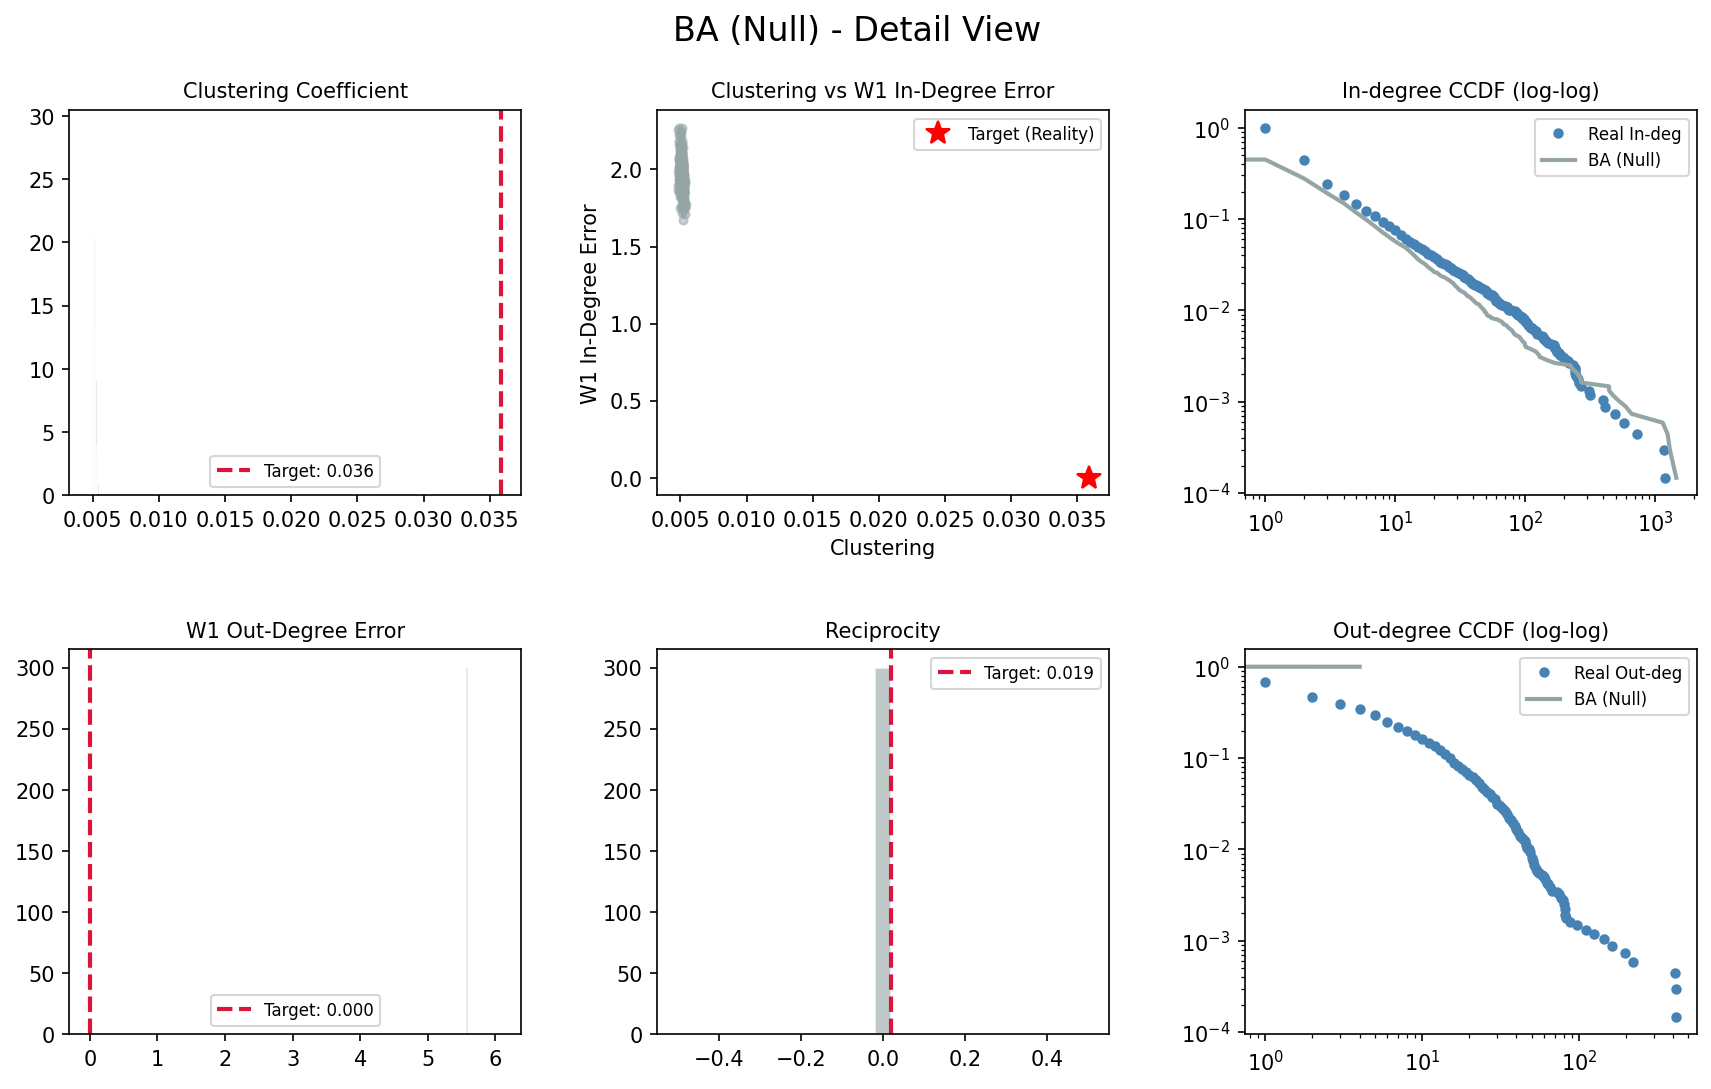
\includegraphics[width=\linewidth]{Imagenes/summary_BA_Null.png}
			\end{column}
		\end{columns}
		\vspace{3mm}
		\begin{itemize}
			\small
			\item \textbf{El éxito de las Micro-Dinámicas:} El modelo \textit{Copying} es el ganador absoluto modelando la popularidad extrema ($p=0.252$ en prueba de Max Hub).
			\item \textbf{Conclusión:} PyPI crece mediante un proceso mimético. Los desarrolladores no eligen dependencias al azar o solo por popularidad (BA); miran el código de otros y \textbf{copian} sus árboles de dependencias.
		\end{itemize}
	\end{frame}
	
	%---------------------------------------------------------
	% DIAPOSITIVA 2: BTER vs SBM_PA
	%---------------------------------------------------------
	\begin{frame}{Macro-Estructura: El Reto de las Comunidades}
		\begin{columns}
			\begin{column}{0.48\textwidth}
				\centering
				\textbf{Modelo BTER} \\
				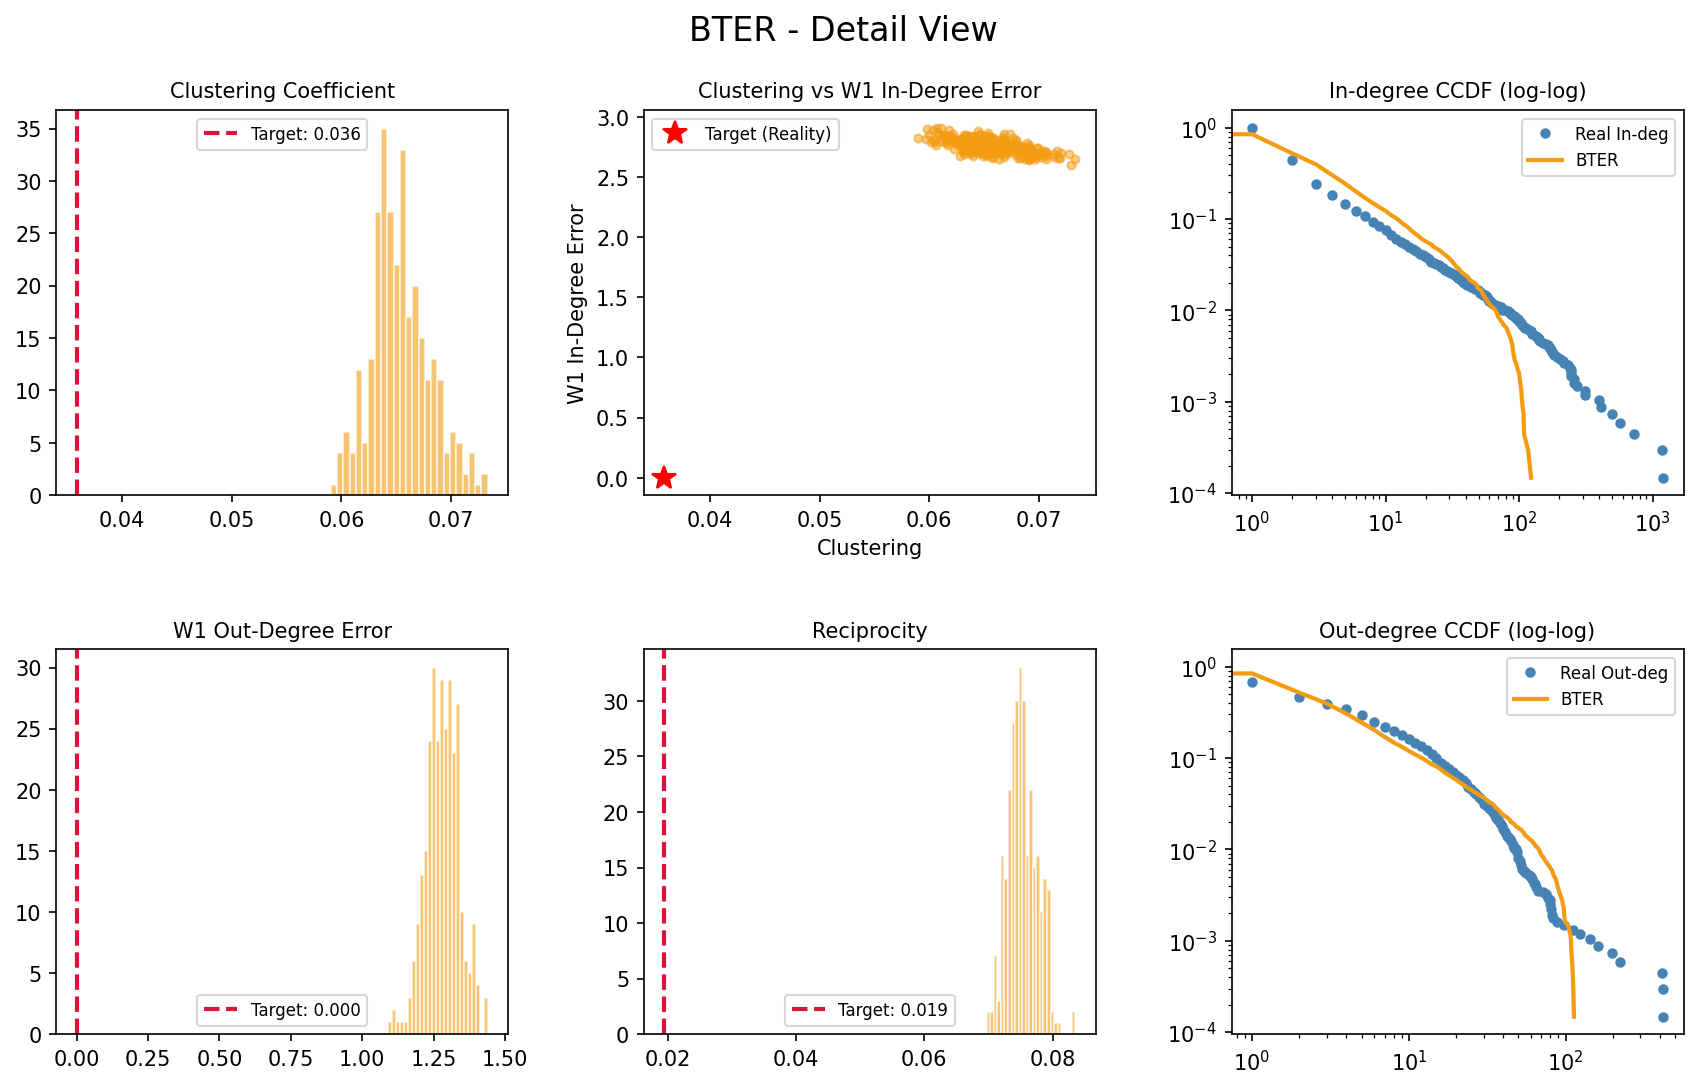
\includegraphics[width=\linewidth]{Imagenes/summary_BTER.png}
			\end{column}
			\begin{column}{0.48\textwidth}
				\centering
				\textbf{Modelo SBM + PA} \\
				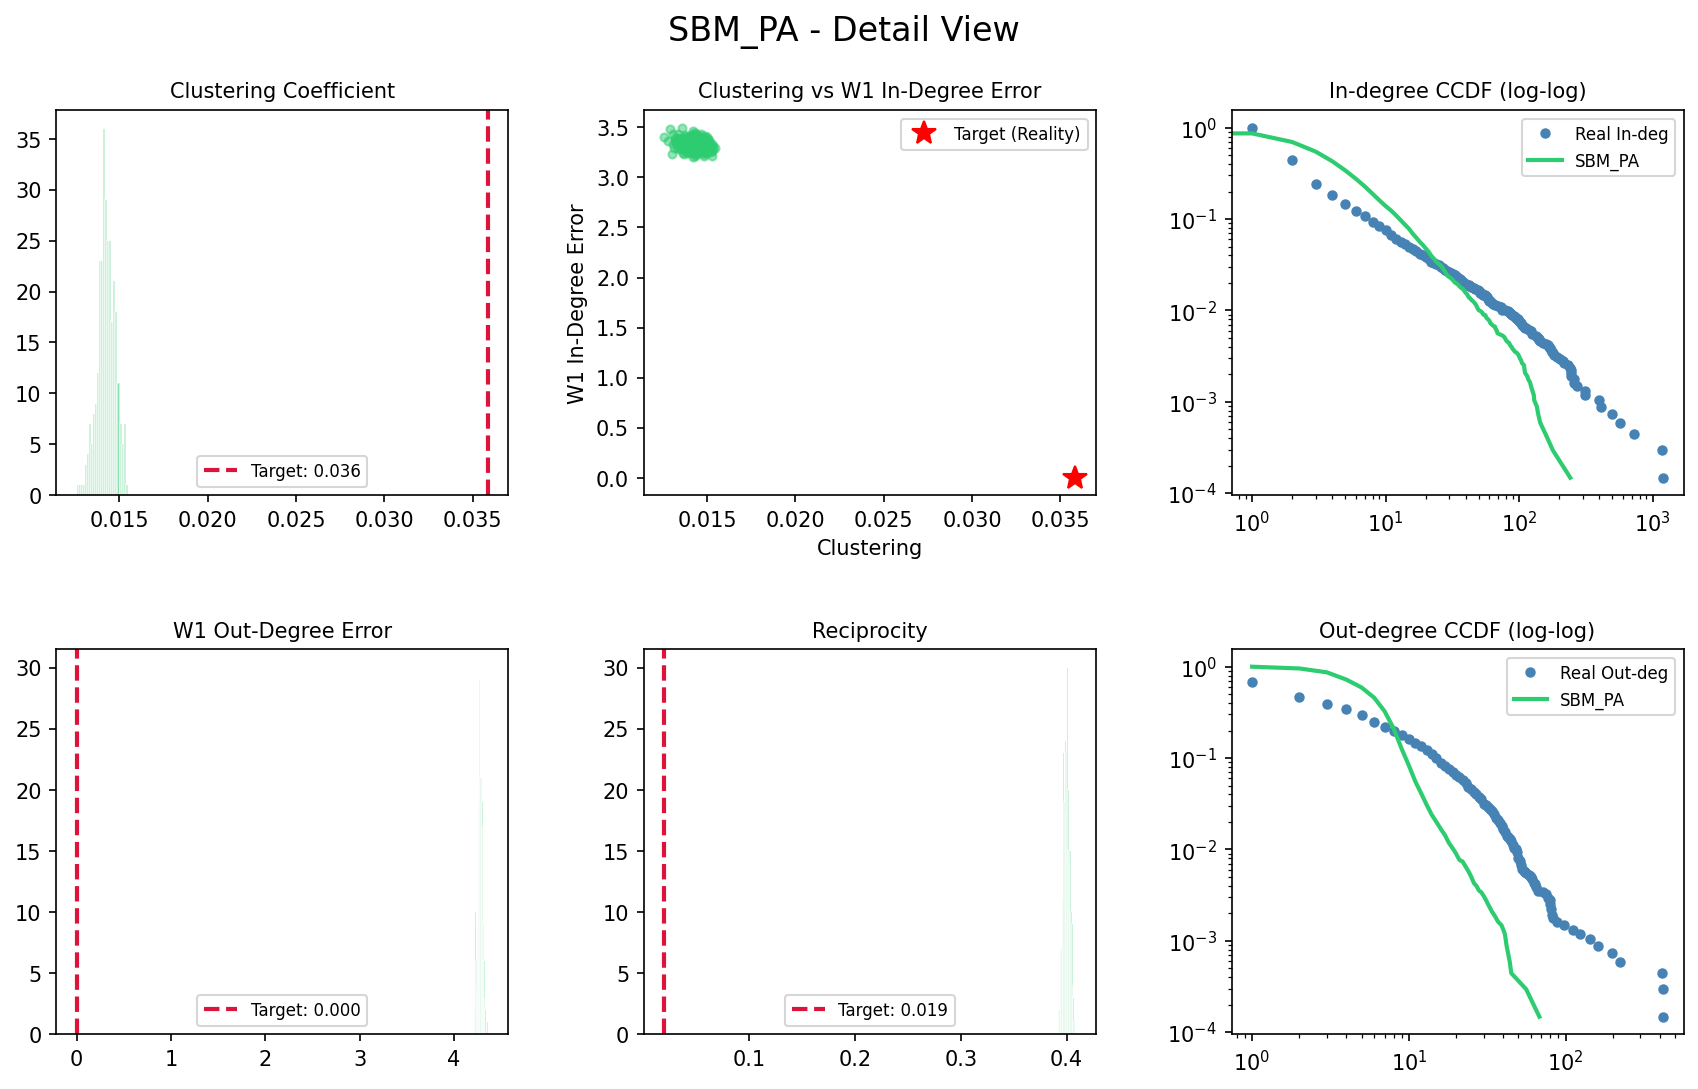
\includegraphics[width=\linewidth]{Imagenes/summary_SBM_PA.png}
			\end{column}
		\end{columns}
		\vspace{3mm}
		\begin{itemize}
			\small
			\item \textbf{El dilema estructural:} BTER logra capturar el \textit{clustering} agrupando nodos en bloques densos, pero al forzar esta estructura destruye la asortatividad humana.
			\item \textbf{Conclusión:} Forzar matemáticamente la creación de comunidades (como intenta SBM\_PA) interfiere con el crecimiento orgánico de la red, generando tasas irreales de reciprocidad.
		\end{itemize}
	\end{frame}
	
	%---------------------------------------------------------
	% DIAPOSITIVA 3: Kronecker vs ERGM
	%---------------------------------------------------------
	\begin{frame}{Rigidez Matemática vs. Especialización Estadística}
		\begin{columns}
			\begin{column}{0.48\textwidth}
				\centering
				\textbf{Grafo Estocástico de Kronecker} \\
				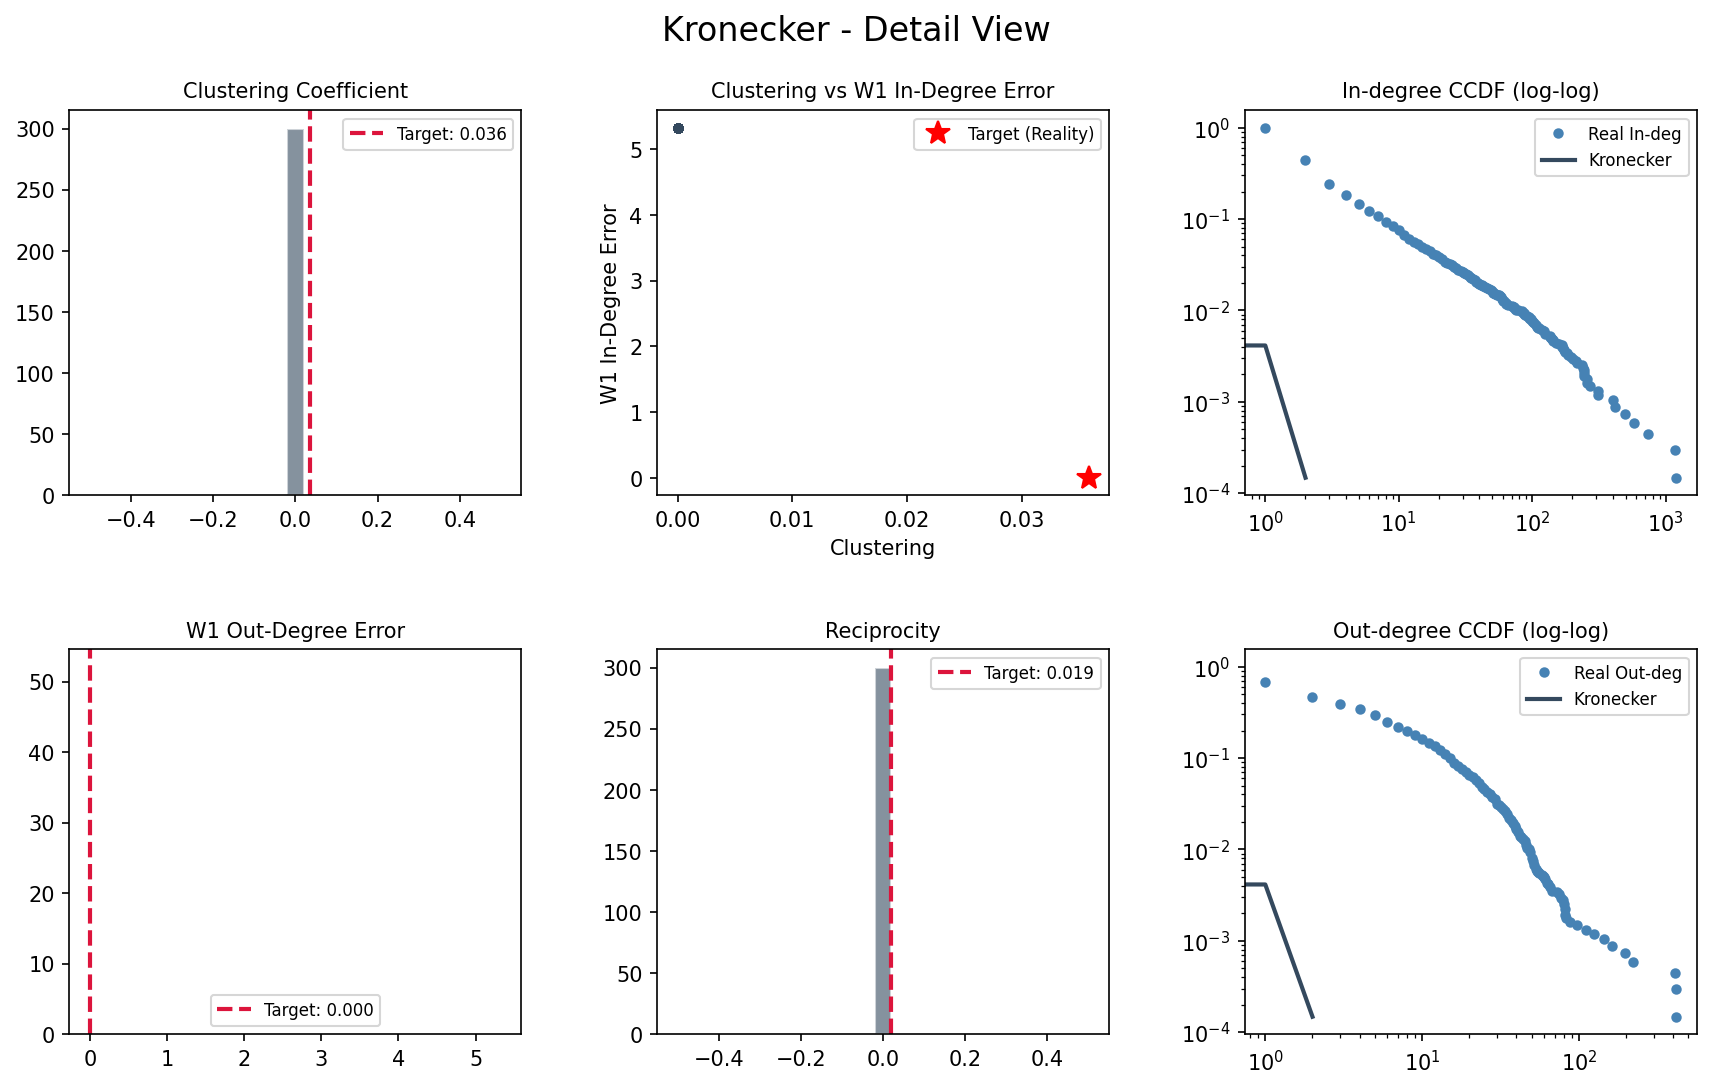
\includegraphics[width=\linewidth]{Imagenes/summary_Kronecker.png}
			\end{column}
			\begin{column}{0.48\textwidth}
				\centering
				\textbf{Modelo ERGM} \\
				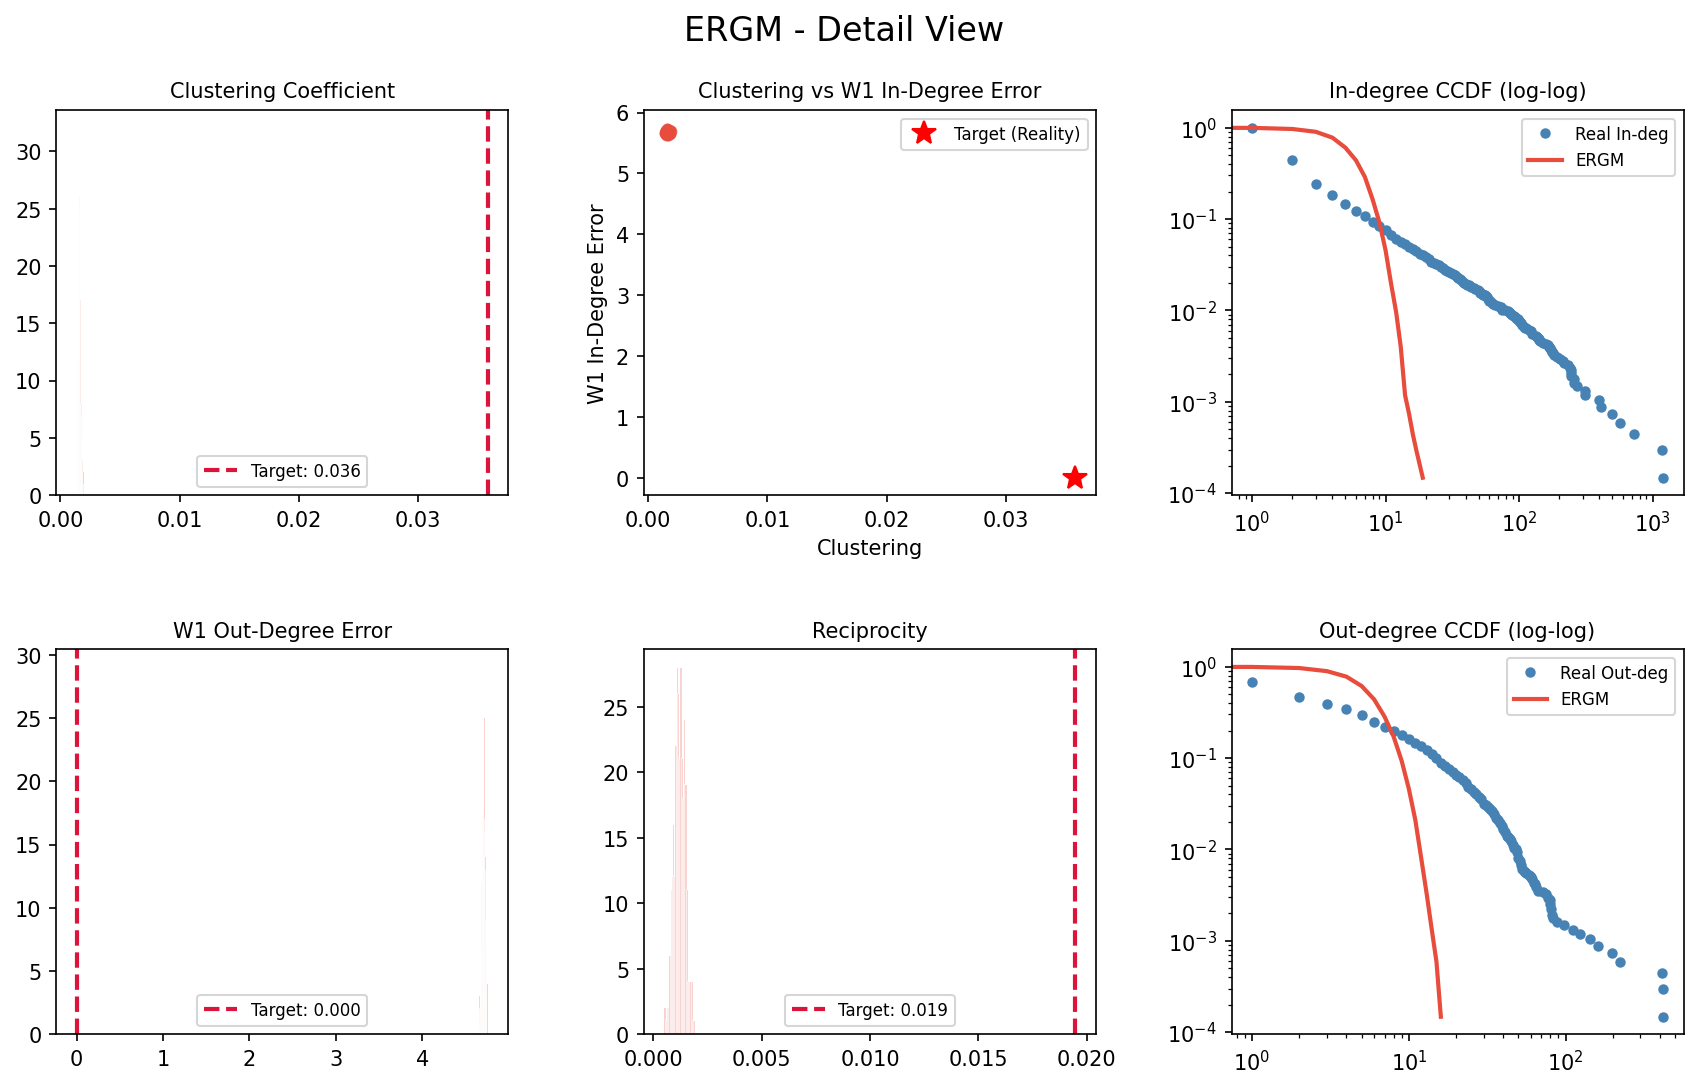
\includegraphics[width=\linewidth]{Imagenes/summary_ERGM.png}
			\end{column}
		\end{columns}
		\vspace{3mm}
		\begin{itemize}
			\small
			\item \textbf{El efecto escalera:} La multiplicación matricial fractal de Kronecker es demasiado rígida y discreta para modelar el desorden orgánico del software.
			\item \textbf{Conclusión:} Aunque técnicas avanzadas como ERGM (MCMC) pueden calibrar métricas globales exactas (clavando la reciprocidad real), son incapaces de simular la evolución natural de las colas pesadas.
		\end{itemize}
	\end{frame}
	
	%---------------------------------------------------------
	% DIAPOSITIVA 4: Bianconi vs ER (Veredicto)
	%---------------------------------------------------------
	\begin{frame}{Aptitud, Aleatoriedad y el Veredicto Final}
		\begin{columns}
			\begin{column}{0.48\textwidth}
				\centering
				\textbf{Modelo Bianconi-Barabási} \\
				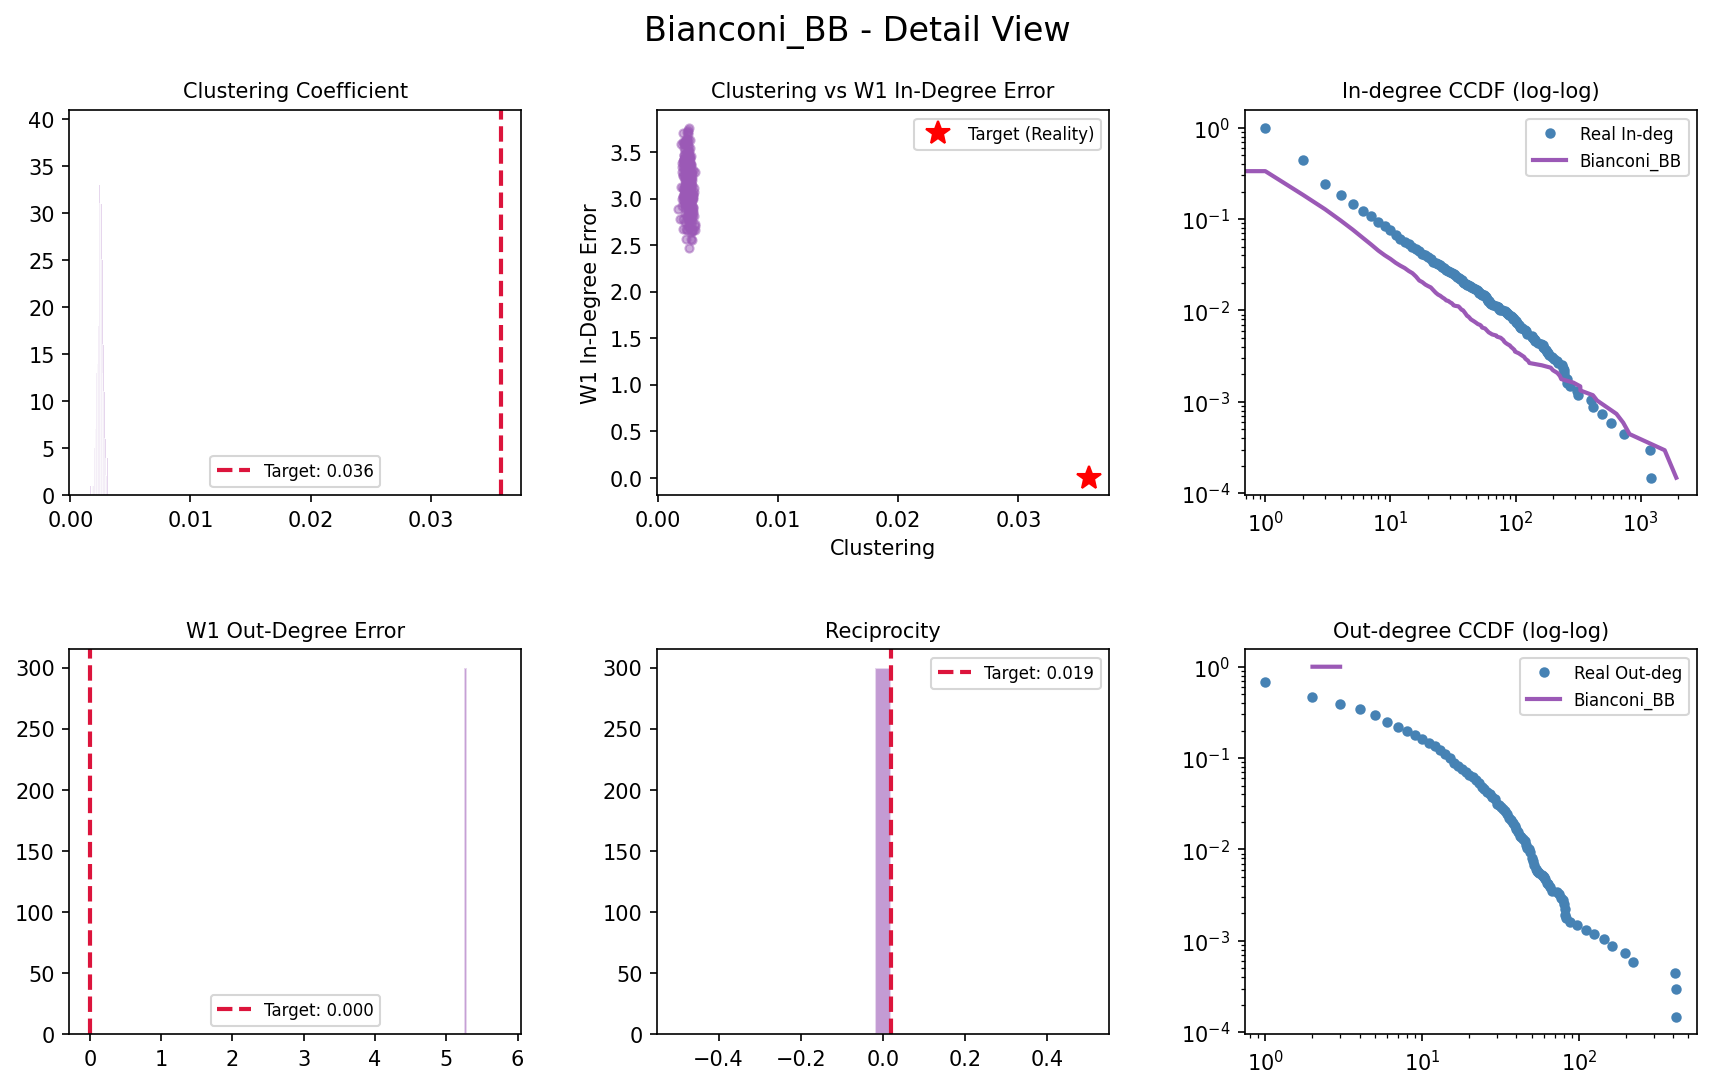
\includegraphics[width=\linewidth]{Imagenes/summary_Bianconi_BB.png}
			\end{column}
			\begin{column}{0.48\textwidth}
				\centering
				\textbf{Modelo Erdős–Rényi (Nulo)} \\
				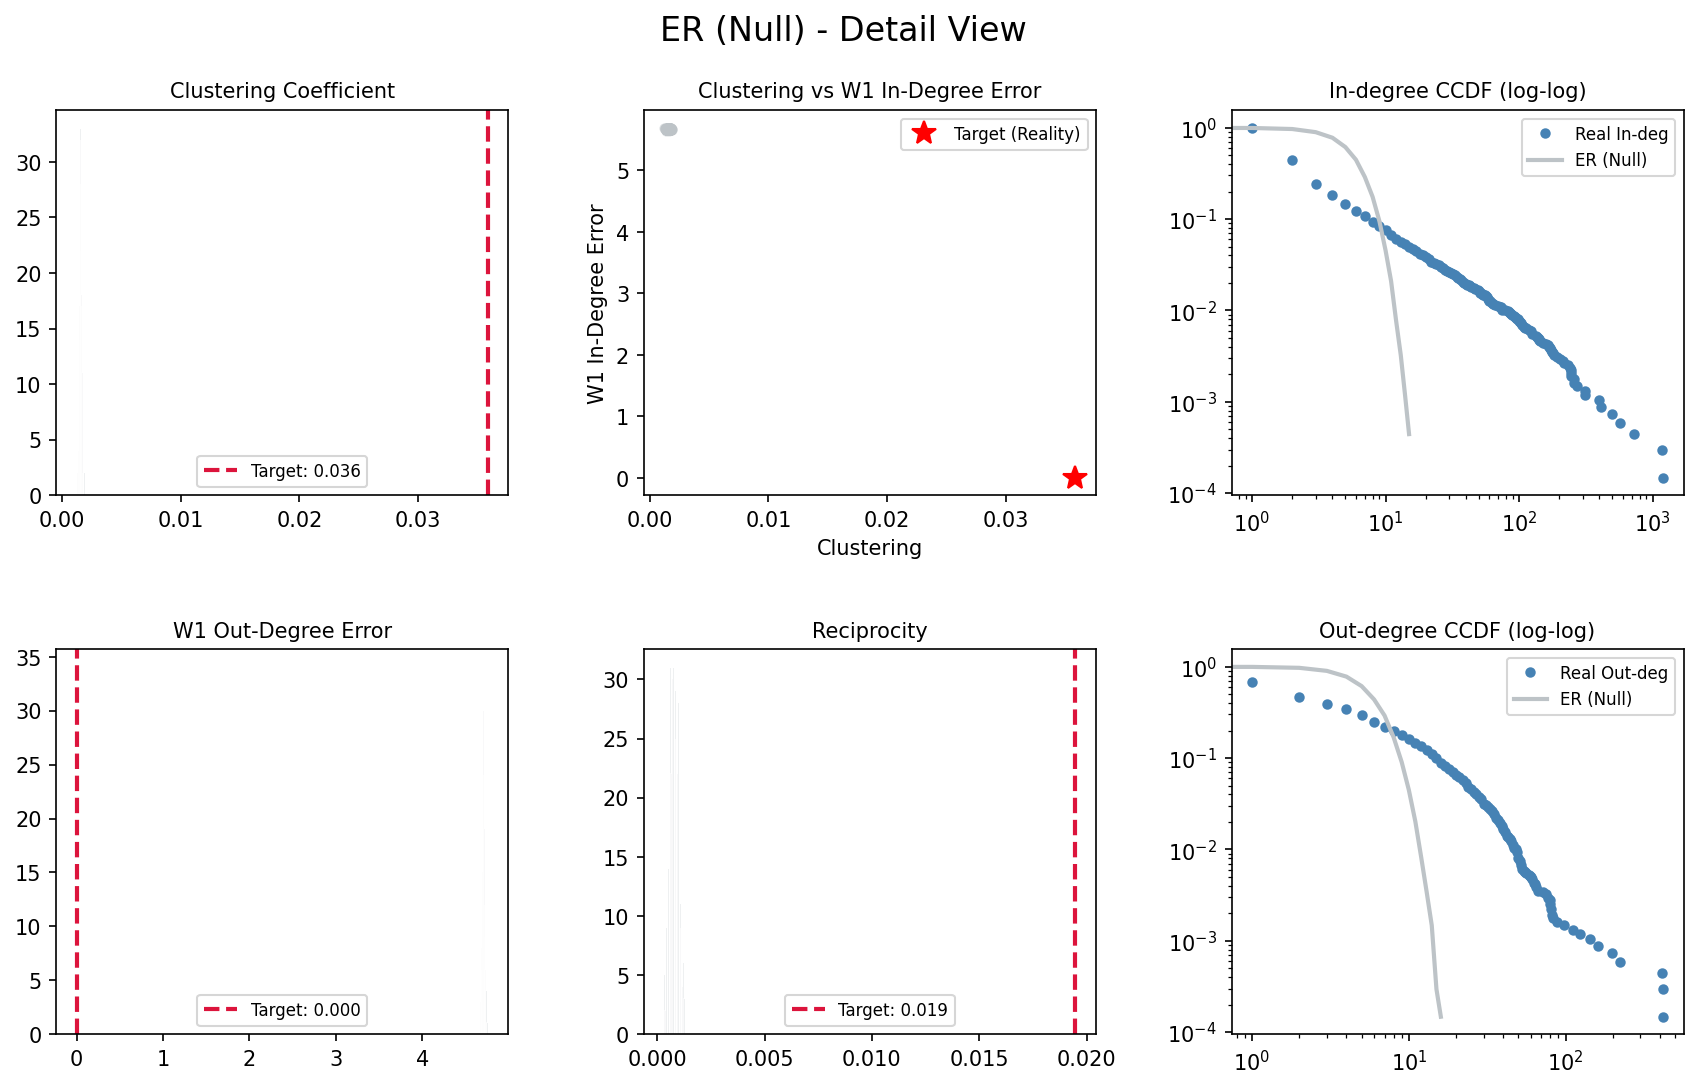
\includegraphics[width=\linewidth]{Imagenes/summary_ER_Null.png}
			\end{column}
		\end{columns}
		\vspace{3mm}
		\begin{itemize}
			\small
			\item \textbf{El límite del crecimiento:} Añadir "Aptitud" o calidad intrínseca al paquete (Bianconi) mejora la precisión frente al puro azar (ER), pero no logra superar a la simple dinámica de copia.
			\item \textbf{Veredicto Final:} La red PyPI exige un modelo híbrido. Crece de manera orgánica e infecciosa (creando mega-hubs por copia), pero se organiza y restringe bajo la lógica disasortativa de la ingeniería de software.
		\end{itemize}
	\end{frame}
	

\end{document}